
\documentclass[11pt]{article}
\usepackage[left=4mm, right=4mm, top=3mm, bottom=7mm,paperwidth=140mm, paperheight=297mm]{geometry}

\usepackage[utf8x]{inputenc}
\usepackage{amssymb, amsfonts, amsmath}
\usepackage{xcolor}
\usepackage[e]{esvect}
\usepackage{floatrow} % allows to insert pictures into proofs and theorems
\usepackage{cancel}
\usepackage{graphicx}
\usepackage{tabularx}
\usepackage{mwe} % for blindtext and example-image-a in example
\usepackage{wrapfig}
\usepackage{framed}
\usepackage{booktabs}
\usepackage[english,german]{babel} 
\usepackage{array}
\usepackage{enumitem}
\usepackage{float}
\usepackage{cancel}
\usepackage{multirow}
\usepackage{multicol}

% Style Sheet
% use greek letters for phi and epsilon
\renewcommand{\phi}{\varphi}
\renewcommand{\epsilon}{\varepsilon}

% bolds math symbols
\newcommand{\bs}{\boldsymbol}
% Shortcut to write caligraphic math symbols
\newcommand{\mc}{\mathcal}
% norm
\newcommand{\norm}[1]{\left| \!\:\! \left| #1 \right| \!\:\! \right|}

% some shortcuts
\newcommand{\ds}{\displaystyle}
\newcommand{\arr}{\rightarrow}
\newcommand{\Arr}{\Rightarrow}
\newcommand{\LRA}{\Leftrightarrow}
\newcommand{\LLRA}{\Longleftrightarrow}
\newcommand{\nop}[1]{}
\newcommand{\rank}{\operatorname{rank}}
\newcommand{\cond}{\operatorname{cond}}
\newcommand{\grad}{\operatorname{grad}}
\newcommand{\argmin}{\mathop{\mathrm{argmin}}}
\newcommand{\argmax}{\mathop{\mathrm{argmax}}}
\newcommand{\mx}{\mathop{\mathrm{max}}}
\newcommand{\bigcupdot}{\bigcup \hspace{-0.35cm} \cdot}

\newcommand*\conj[1]{\overline{#1}}
\newcommand*\abs[1]{\vert #1 \vert}
\newcommand*\floor[1]{\lfloor #1 \rfloor}
\newcommand*\set[1]{\lbrace #1 \rbrace}
\newcommand{\eqdef}{\xlongequal{\text{def}}}
\newcommand{\lims}{\lim_{x \rightarrow x_0}}
\newcommand*\seq[1]{(#1)_{n = 0}^{\infty}}
\newcommand{\sinx}{sin(x)}
\newcommand{\siny}{sin(y)}
\newcommand{\cosx}{cos(x)}
\newcommand{\cosy}{cos(y)}
\newcommand{\tanx}{tan(x)}
\newcommand{\tany}{tan(y)}

% stuff for integrals
\newcommand{\intl}{\int\limits}
\newcommand{\rmd}{\mathrm{d}}
\newcommand{\rmD}{\mathrm{D}}

% number sets
\newcommand{\R}{\mathbb{R}}
\newcommand{\E}{\mathbb{E}}
\newcommand{\Z}{\mathbb{Z}}
\newcommand{\N}{\mathbb{N}}
\newcommand{\Q}{\mathbb{Q}}
\newcommand{\C}{\mathbb{C}}
\newcommand{\K}{\mathbb{K}}
\newcommand{\M}{\mathbb{M}}

% big-o notation
\newcommand{\bigO}{\mathcal{O}}

% 'with' in set notation
\newcommand{\with}{\;|\;}

% hyperref
\usepackage[colorlinks=false,pdfborder = {0 0 0 0}]{hyperref}


\colorlet{shadecolor}{orange!15}
\columnsep24pt
\columnseprule0.1pt

\setlength{\parindent}{0px}
\setlength{\parskip}{5px}
\setlength{\parsep}{0px}
\setcounter{secnumdepth}{4}

%% Redefine the \paragraph command:
\makeatletter
\renewcommand\paragraph{\@startsection{paragraph}{4}{0mm}%
	{-\baselineskip}%
	{0.5\baselineskip}%
	{\normalfont\bfseries}%
}%
\makeatother 

% algorithms
\usepackage{algorithmic}
\usepackage{algorithm}
\algsetup{linenodelimiter=}

% listings
\definecolor{darkgreen}{RGB}{0,127,14}
\definecolor{purple}{RGB}{75,0,130}
\usepackage{listings}


\usepackage{listings}
\usepackage{xcolor}
\lstset { %
    language=Pascal,
    backgroundcolor=\color{black!5}, % set backgroundcolor
    basicstyle=\footnotesize,% basic font setting
    escapeinside={!}{!},
    tabsize=2,
}

\def\doubleunderline#1{\underline{\underline{#1}}}

% theorem package
\usepackage{amsthm}
\usepackage{thmtools}
\newtheoremstyle{my-thm-style}% name
{6pt}% Space above
{5pt}% Space below
{}% Body font
{}% Indent amount
{\bfseries}% Theorem head font
{}% Punctuation after theorem head
{3pt}% Space after theorem head
{}% Theorem head spec (can be left empty, meaning `normal')

\definecolor{grey}{RGB}{40, 55, 71}
\definecolor{blue}{RGB}{93, 173, 226}
\definecolor{green}{RGB}{130, 224, 170}
\definecolor{red}{RGB}{229, 115, 115 }

\declaretheoremstyle[
headfont=\normalfont\bfseries,
notefont=\mdseries, notebraces={(}{)},
bodyfont=\normalfont,
postheadspace=8pt,
spaceabove=1pt,
mdframed={
  skipabove=2pt,
  skipbelow=2pt,
  hidealllines=false,
  backgroundcolor={blue!10},
  innerleftmargin=2pt,
  innerrightmargin=2pt}
]{def}

\declaretheoremstyle[
headfont=\normalfont\bfseries,
notefont=\mdseries, notebraces={(}{)},
bodyfont=\normalfont,
postheadspace=8pt,
spaceabove=1pt,
mdframed={
  skipabove=2pt,
  skipbelow=2pt,
  hidealllines=false,
  backgroundcolor={grey!10},
  innerleftmargin=2pt,
  innerrightmargin=2pt}
]{sat}

\declaretheoremstyle[
headfont=\normalfont\bfseries,
notefont=\mdseries, notebraces={(}{)},
bodyfont=\normalfont,
postheadspace=8pt,
spaceabove=1pt,
mdframed={
  skipabove=2pt,
  skipbelow=2pt,
  hidealllines=false,
  backgroundcolor={green!10},
  innerleftmargin=2pt,
  innerrightmargin=2pt}
]{lem}

\declaretheoremstyle[
headfont=\normalfont\bfseries,
notefont=\mdseries, notebraces={(}{)},
bodyfont=\normalfont,
postheadspace=8pt,
spaceabove=1pt,
mdframed={
  skipabove=2pt,
  skipbelow=2pt,
  hidealllines=false,
  backgroundcolor={green!0},
  innerleftmargin=2pt,
  innerrightmargin=2pt}
]{kor}

\declaretheorem[style=def, name=Def. , numberwithin=section]{definition}
\declaretheorem[style=sat, name=Satz, numberwithin=section]{satz}
\declaretheorem[style=lem, name=Lemma, numberwithin=section]{lemma}
\declaretheorem[style=kor, name=Korollar, numberwithin=section]{korollar}



%%%%%
\begin{document}
	
\setcounter{page}{1}
\setcounter{tocdepth}{2}

\title{Analysis I, ETH, D-INFK}
<<<<<<< HEAD
\author{Miles Straessle}
=======
\author{Miles Strässle}
>>>>>>> 4851b202d1f20c0a2c90b1ba1226d4f09fce89dc
\date{\today}
\maketitle
%\tableofcontents


% Use compiler for 3x1 Format on A4 Page, ask Author
% include the individual chapters
% \input{kap<n>.tex}
%\clearpage

%% Multiline-Comment
% \ifx true false
% ...
% \fi


\part{Zusammenfassung}

\section{Folgen}
%%%%%%%%%%

\subsection{Definitionen}
\begin{description}[noitemsep,topsep=0pt]
	\item[konvergent] $\lim_{x \to \infty} a_n$ existiert \index{konvergent}
	\item[divergent] $\lim_{x \to \infty} a_n$ existiert nicht \index{divergent}
	\item[Nullfolge] $\lim_{x \to \infty} a_n = 0$ gilt \index{Nullfolge}
	\item[beschränkt] Es gibt $C_1, C_2$, so dass gilt $C_1 \leq a_n \leq C_2$
	bzw. $C$ gibt, so dass $|a_n| \leq C$
	\item[unbeschränkt] falls $(a_n)$ nicht beschränkt ist. Unbeschränkte folgen
	sind stets \underline{divergent}
	\item[monoton wachsend] $a_n \leq a_{n+1} \quad \forall n \in \N$ \index{monoton}
	\item[streng monoton wachsend] $a_n < a_{n+1} \quad \forall n \in \N$
	\item[monoton fallend] $a_n \geq a_{n+1} \quad \forall n \in \N$
	\item[streng monoton fallend] $a_n > a_{n+1} \quad \forall n \in \N$
	\item[alternierend] die Vorzeichen der Folgenglieder wechseln sich ab
	\item[bestimmt divergent / uneigentlich konvergent] es gilt $\lim_{n \to
		\infty} a_n = \pm \infty$
\end{description}

\begin{definition}[Grenzwert] \index{Grenzwert}
	\begin{align*}
		\lim_{n \to \infty} a_n = a & \Leftrightarrow a_n \to a \\
		& \Leftrightarrow \forall \epsilon > 0 \exists n_0 \in \N \forall n \geq n_0:
		|a_n - a| < \epsilon
	\end{align*}
\end{definition}

\begin{definition}[Teilfolge] \index{Teilfolge}
	Werden von einer Folge beliebig viele Glieder weggelassen, aber nur so viele,
	dass noch unendlich viele übrigbleiben, so erhält man eine Teilfolge.
\end{definition}

\begin{definition}[Häufungspunkt] \index{Häufungspunkt}
	$a$ ist Häufungspunkt der Folge $(a_n)$, wenn in jeder Umgebung von $a$
	unendlich viele Folgeglieder liegen. Das ist äquivalent damit, dass $a$ der
	Limes einer Teilfolge von $(a_n)$ ist.
\end{definition}

\begin{definition}[Limes superior / Limes inferior] \index{$\limsup$}\index{$\liminf$}
	Ist $(a_n)$ eine beschränkte Folge, so heisst der grösste Häufungspunkt Limes
	superior ($\limsup_{n \to \infty} a_n$ oder $\overline{\lim}_{n \to \infty}
	a_n$). Der kleinste Häufungspunkt ist der Limes inferior ($\liminf_{n \to
		\infty} a_n$ oder $\underline{\lim}_{n \to \infty} a_n$)
\end{definition}


\subsection{Rechnen mit Eigenschaften}
Addition:
\begin{itemize}[noitemsep,topsep=0pt]
	\item $(a_n), (b_n)$ konvergiert $\Rightarrow (a_n + b_n)$ konvergiert
	\item $(a_n)$ konvergiert, $(b_n)$ divergent $\Rightarrow (a_n + b_n)$
	divergent
	\item $(a_n)$ beschränkt, $(b_n)$ beschränkt $\Rightarrow (a_n + b_n)$
	beschränkt
	\item $(a_n)$ beschränkt, $(b_n)$ unbeschränkt $\Rightarrow (a_n + b_n)$
	unbeschränkt
	\item $(a_n)$ beschränkt, $(b_n) \to \pm \infty \Rightarrow (a_n + b_n) \to
	\pm \infty$
	\item $(a_n) \to \infty$, $(b_n) \to \infty \Rightarrow (a_n + b_n) \to \infty$
	\item $(a_n) \to -\infty$, $(b_n) \to -\infty \Rightarrow (a_n + b_n) \to
	-\infty$
\end{itemize}

Produkt:
\begin{itemize}[noitemsep,topsep=0pt]
	\item $(a_n)$ Nullfolge, $(b_n)$ beschränkt $\Rightarrow (a_n b_n)$ Nullfolge
	\item $(a_n)$ konvergent, $(b_n)$ beschränkt $\Rightarrow (a_n b_n)$
	beschränkt
	\item $(a_n)$ konvergent, $(b_n)$ konvergent $\Rightarrow (a_n b_n)$
	konvergent
	\item $(a_n)$ konvergent gegen $a \neq 0$, $(b_n)$ divergent $\Rightarrow
	(a_n b_n)$ divergent
\end{itemize}

\subsection{Rechnen mit Grenzwerten}
$\lim_{n \to \infty} a_n = a$, $\lim_{n \to \infty} b_n = b$\\
\emph{\underline{Achtung!} Untenstehendes gilt \underline{nur} wenn die Grenzwerte von $a_n$ und $b_n$ existieren. (Nicht $0$ oder $\inf$ sind.)}
\begin{itemize}[noitemsep,topsep=0pt]
	\item $\lim_{n \to \infty} (a_n \pm b_n) = a \pm b$
	\item $\lim_{n \to \infty} (c \cdot a_n) = c \cdot a$
	\item $\lim_{n \to \infty} (a_n b_n) = ab$
	\item \underline{Achtung:} $\lim_{n \to \infty} (a_n)^c = (\lim_{n \to
		\infty} a_n)^c$, nur wenn $c \neq n$
	\item $\lim_{n \to \infty} \frac{a_n}{b_n} = \frac{a}{b}, \quad (b_n)$ keine
	Nullfolge
\end{itemize}

\subsection{Hilfsmittel}
\textbf{Bernoullische Ungleichung}: Für $x \geq -1$ und $n \in \N$
\[
(1+x)^n \geq 1 + nx
\]


\textbf{Vergleich von Folgen}: weiter rechts stehende Werte gehen schneller nach
$\infty$
\[
1, \quad \ln n, \quad n^\alpha \; (\alpha > 0), \quad q^n \; (q > 1), \quad n!,
\quad n^n
\]

\textbf{Stirlingformel}:
\[
n! \approx \sqrt{2 \pi n} \left (\frac{n}{e} \right )^n
\Rightarrow \left ( \frac{n}{e} \right )^n \sqrt{2 \pi n} \leq n! \leq \left (
\frac{n}{e} \right )^n \sqrt{2 \pi n} \cdot e^\frac{12}{n}
\]

\subsection{Konvergenzkriterien}\index{Konvergenzkriterien}
\begin{align*}
	a_n \to a \Leftrightarrow a_n - a \to 0 \Leftrightarrow |a_n - a| \to 0
\end{align*}

\begin{itemize}[leftmargin=*,noitemsep,topsep=0pt]	
	\item Ist $\lim_{n \to \infty} a_n = a$, so ist der Limes $a$ einziger
	Häufungspunkt der Folge $(a_n)$ und jede Teilfolge konvergiert auch gegen $a$.
	
	\textbf{Beispiel:} Wegen $\left( 1 + \frac{1}{n} \right)^n \to e$, so gilt auch
	$\left( 1 + \frac{1}{2n} \right)^{2n} \to e$
	
	\item Hat die Folge zwei verschiedene Häufungspunkte, so ist die Folge sicher
	divergent.
	
	\item Ist die Folge monoton steigend und nach oben beschränkt, dann existiert \\
	$\lim_{n \to \infty} a_n$. Ist die Folge monoton fallend und nach unten
	beschränkt, dann existiert $\lim_{n \to \infty} a_n$
	
	\item Konvergiert $\sum_{n=0}^\infty a_n$, so ist $\lim_{n \to \infty} a_n =
	0$\\
	Damit kann die Regeln für Reihen verwenden. Siehe Grenzwerte von Reihen.
	
	\item Gibt es eine Funktion $f$ mit $f(n) = a_n$ und $\lim_{x \to \infty} f(x)
	= a$, so gilt auch $\lim_{n \to \infty} a_n = a$.\\
	Damit kann man zum Beispiel die Regel von \underline{l'Hospital} und die
	restlichen Methoden anwenden. Siehe Grenzwerte von Funktionen.\\
	\underline{Achtung:} Es kann sein, dass $f$ keinen Grenzwert besitzt, aber
	$(a_n)$ schon.
	
	\item \textbf{Einschliessungskriterium}: Sind $(a_n), (b_n), (c_n)$ Folgen mit
	$a_n \leq b_n \leq c_n$ und haben $(a_n), (c_n)$ den gleichen Grenzwert $a$, so
	konvergiert auch $(b_n)$ nach $a$.
\end{itemize}
\newpage
\subsection{Tipps \& Beispiele}
\subsubsection{Brüche}
$\lim_{n \to \infty} \frac{n^2 + \ln n}{\sqrt{n^4 - n^3}}$

Bei Brüchen empfiehlt es sich den am stärksten wachsenden Teil (das am
schnellsten wachsende $n$) zu kürzen. In diesem Fall ist es das $n^4$ in der
Wurzel, also $n^2$.

\begin{align*}
	\ldots &= \lim_{n \to \infty} \frac{n^2 + \ln n}{\sqrt{n^4 - n^3}}
	\cdot \frac{\frac{1}{n^2}}{\frac{1}{n^2}} = \lim_{n \to \infty} \frac{n^2 + \ln
		n}{n^2 \sqrt{1 - \frac{1}{n}}} \cdot \frac{\frac{1}{n^2}}{\frac{1}{n^2}} \\
	&= \lim_{n \to \infty} \frac{1 + \frac{\ln n}{n^2}}{\sqrt{1 - \frac{1}{n}}}
	= \frac{1 + 0}{\sqrt{1 - 0}} = 0
\end{align*}

\subsubsection{l'Hospital für Folgen (Folge als Funktion)}
$\lim_{n \to \infty} \frac{\ln n}{n^2}$

Die Funktion $f(x) = \frac{\ln x}{x^2}$ entspricht unseren Folgegliedern ($f(n)
= a_n = \frac{\ln n}{n^2}$). Für $n \to \infty$ hat der Nenner und der Zähler
den Grenzwert $\infty$, also wenden wir die Regel von l'Hospital an.

\begin{align*}
	\ldots &= \lim_{x \to \infty} \frac{(\ln x)'}{(x^2)'} = \lim_{x \to \infty}
	\frac{\frac{1}{x}}{2x} = \lim_{x \to \infty} \frac{1}{x^2} = 0
\end{align*}

Somit geht auch die Folge gegen 0.

\subsubsection{Wurzeln}
$\lim_{n \to \infty} (\sqrt{n^2 + an + 1} - \sqrt{n^2 + 1})$

Hier wendet man die dritte binomische Formel an, um den grenzwert zu berechnen.
Die einzelnen Terme streben jeweils gegen $\infty$ und $\infty - \infty$ kann
nicht berechnet werden.

\underline{Achtung} auf die Vorzeichen beim Anwenden der Regel!

\begin{align*}
	&= \lim_{n \to \infty} (\sqrt{n^2 + an + 1} - \sqrt{n^2 + 1}) \cdot
	\left(\frac{\sqrt{n^2 + an + 1} + \sqrt{n^2 + 1}}{\sqrt{n^2 + an + 1} +
		\sqrt{n^2 + 1}} \right) \\
	&= \lim_{n \to \infty} \frac{(n^2 + an + 1) - (n^2 + 1)}{\sqrt{n^2 + an + 1} +
		\sqrt{n^2 + 1}} \\
	&= \lim_{n \to \infty} \frac{an}{\sqrt{n^2 + an + 1} + \sqrt{n^2 + 1}} 
\end{align*}

nun verwenden wir den Tipp für Brüche und kürzen das $n$ heraus

\begin{align*}
	\ldots &= \lim_{n \to \infty} \frac{a}{\sqrt{1 + \frac{a}{n} + \frac{1}{n^2}} +
		\sqrt{1 + \frac{1}{n^2}}} = \frac{a}{1 + 1} = \frac{a}{2}
\end{align*}

\newpage
\subsection{Cauchy-Folgen}\index{Cauchy-Folge}
\begin{definition}[Cauchy-Folge]
	Sei $(a_n)_{n \in \N}$ eine Folge in $\R$. $(a_n)_{n \in \N}$ heisst \textbf{Cauchy-Folge}, falls gilt
	\begin{align*}
		\forall \epsilon > 0 \; \exists n_n = n_0(\epsilon) \in \N \; \forall n, l \geq n_0: |a_n - a_l| < \epsilon
	\end{align*}
\end{definition}

Die Definition sagt grundsätzlich aus, dass ab einem $n_0(\epsilon)$ (also einem Anfang $n_0$, der abhängig von $\epsilon$ ist)
die Folgeglieder nur noch $\epsilon$ Abstand zu einander haben. Also der Abstand beliebig klein wird zwischen Folgegliedern.

\begin{satz}[Cauchy-Kriterium]
	Für $(a_n)_{n \in \N} \subset \R$ sind äquivalent:
	\begin{itemize}
		\item $(a_n)_{n \in \N}$ ist konvergent
		\item $(a_n)_{n \in \N}$ ist Cauchy-Folge
	\end{itemize}
\end{satz}



\section{Reihen}

\subsection{Definitionen}
Eine Reihe $\sum_{n = 1}^\infty a_n$ ist \underline{konvergent} mit Grenzwert
$s$, wenn die Folge der \underline{Partialsummen} $(S_m)$, $S_m :=
\sum_{n=1}^m a_n$ gegen $s$ konvergiert. Also wenn gilt: $S_m \to s$.

\begin{definition}[$\epsilon$-Kriterium]
	$\forall \epsilon > 0 \; \exists n_0 \in \N \; \forall m \geq n_0: \left|
	\sum_{n=1}^m a_n - s \right| < \epsilon$
\end{definition}

\begin{definition}[Absolute Konvergenz]\index{Konvergenz}
	Wenn auch die Reihe der Absolutbeträge $\sum_{n=1}^\infty |a_n|$ konvergiert, so
	heisst die Reihe absolut konvergent. Aus der absoluten Konvergenz folgt
	Konvergenz. Der Umkehrschluss ist nicht möglich.
\end{definition}

\subsection{Rechenregeln Reihen}
Für \underline{konvergente} Reihen gilt:
\[
\sum_{n=1}^\infty a_n = A, \sum_{n=1}^\infty b_n = B \Rightarrow
\sum_{n=1}^\infty (\alpha a_n + \beta b_n) = \alpha A + \beta B
\]

\subsection{Konvergenzkriterien}
\begin{tabular}{|l|}
	\hline
	Konvergiert $\sum_{n=1}^\infty a_n$, so ist $\lim_{n \to \infty} a_n = 0$.\\
	Wenn also $\lim_{n \to \infty} a_n \neq 0$, so konvergiert die Reihe
	\underline{nicht}\\
	\hline
\end{tabular}

\begin{table}[H]
	\centering
	\begin{tabular}{|p{4.5cm}|p{3.5cm}|p{4.3cm}|}
		\hline
		& \textbf{Eignung}    & \textbf{Bemerkung}                        \\ \hline
		\textbf{Limes des allgemeinen Glieds}        &                     & zeigt nur Divergenz                       \\ \hline
		\textbf{Majoranten- und Minorantenkriterium} &                     & ersten Glieder spielen keine Rolle        \\ \hline
		\textbf{Quotientenkriterium}                 & $a_n$ mit Faktoren wie $n!$, $a^n$, oder Polynome & gleiche Folgerung wie Wurzelkriterium     \\ \hline
		\textbf{Wurzelkriterium}                     & $a_n = (b_n)^n$     & gleiche Folgerung wie Quotientenkriterium \\ \hline
		\textbf{Leibnitz-Kriterium}                  & $\sin$, $\cos$, $\tan$, $(-1)^n$ &                                           \\ \hline
		\textbf{Absolute Konvergenz}                 & $\sin$, $\cos$, $\tan$, $(-1)^n$   &                                           \\ \hline
		\textbf{Sandwich-Theorem}					 & $\sin$, $\cos$, $\tan$, $(-1)^n$ & \\ \hline
	\end{tabular}
\end{table}
\subsubsection{Reihen Kriterien}
Achtung. Die nachfolgenden Kriterien sagen nur aus, ob die Reihen konvergiert
oder nicht. Sie sagen \underline{nicht} aus, gegen was sie konvergieren!

\paragraph{Quotientenkriterium}
\[
\left| \frac{a_{n+1}}{a_n} \right| \to q. \quad \text{Dann gilt} \begin{cases}
q < 1 & \Rightarrow \sum_{n=1}^\infty a_n \text{ konvergiert absolut} \\
q = 1 & \Rightarrow \text{keine Aussage}\\
q > 1 & \Rightarrow \sum_{n=1}^\infty a_n \text{ divergiert}
\end{cases}
\]

\paragraph{Wurzelkriterium}
\[
\sqrt[n]{\left | a_n \right |} \to q. \quad \text{Dann gilt} \begin{cases}
q < 1 & \Rightarrow \sum_{n=1}^\infty a_n \text{ konvergiert absolut}\\
q = 1 & \Rightarrow \text{keine Aussage}\\
q > 1 & \Rightarrow \sum_{n=1}^\infty a_n \text{ divergiert}
\end{cases}
\]

\paragraph{Leibnizkriterium}
Wenn gilt:
\begin{itemize}
	\item $(a_n)$ ist alternierende Folge, d.h die Vorzeichen wechseln jedes Mal
	\item $a_n \to 0$ oder $|a_n| \to 0$
	\item $(|a_n|)$ ist monoton fallend
\end{itemize}
\ldots dann konvergiert $\sum_{n=1}^\infty a_n$

\paragraph{Majorantenkriterium}
Ist $|a_n| \leq b_n$ und $\sum_{n=1}^\infty b_n$ konvergent, so konvergiert
$\sum_{n=1}^\infty a_n$ absolut.

\paragraph{Minorantenkriterium}
Ist $a_n \geq b_n \geq 0$ und $\sum_{n=1}^\infty b_n$ divergent, so divergiert
$\sum_{n=1}^\infty a_n$

\subsection{Potenzreihe}
Die Potenzreihe hat die allgemeine Form
\[
\sum_{n=0}^\infty a_n (x - x_0)^n
\]

$x_0$ ist der Entwicklungspunkt der Potenzreihe und $(a_n)_{n \in \N}$ eine
beliebige Folge.

\subsubsection{Konvergenzradius}
Die Berechnung des Konvergenzradius ist für solche Reihen einfacher, da der
Faktor $(x - x_0)$ nicht analysiert werden muss. Entsprechend gilt für den
Konvergenzradius $r$:
$r = \frac{1}{\limsup_{n\to\infty} \sqrt[n]{\|a_n\|}}$ (Wurzelkriterium) bzw.
$r = \lim_{n\to\infty} \left | \frac{a_n}{a_{n+1}} \right |$
(Quotientenkriterium).



%%%%%%%%%%

\section{Stetigkeit}

\subsection{Zwischenwertsatz}
Sei $f: [a,b] \to \R$ eine stetige reele Funktion, die auf einem Intervall
definiert ist. Dann existiert zu jedem $u \in [f(a), f(b)]$ (falls $f(a) \leq
f(b)$, sonst $u \in [f(b), f(a)]$) ein $c \in [a,b]$, sodass gilt: $f(c)= u$.

\subsubsection{Beispiel (Fixpunkt)}
Sei $f: [0,1] \to [0,1]$. Zeige: $f$ hat einen Fixpunkt, d.h. es gibt ein $x
\in [0,1]$ derart, dass $f(x) = x$.

Man erzeugt die Funktion $g: [0,1] \to \R, g(x) := f(x) - x$. Es gilt: $f(x) =
x \Leftrightarrow g(x) = 0$, d.h. ein Punkt x ist genau dann ein Fixpunkt von
$f$ wenn er eine Nullstelle von $g$ ist. Es ist zu zeigen, dass $g$ immer eine
Nullstelle auf $[0,1]$ hat. Als Differenz von zwei stetigen Funktionen ist $g$
stetig. Weil ausserdem $f(x) \in [0,1] \; \forall x \in [0,1]$ gilt, ist $g(0)
\geq 0 \geq g(1)$. Da $g$ stetig ist, gibt es daher nach dem Zwischenwertsatz
ein $x \in [0,1]$ mit $g(x) = 0$ und somit gibt es $f(x) = x$.


\subsection{Lipschitz-Stetigkeit}
Es existiert eine Konstante $L\in \mathbb{R}$, sodass:
\begin{equation*}
	|f(x)-f(y)|\leq L|x-y| \quad \forall x,y \in \Omega
\end{equation*}

\emph{Bemerkung:} Ist $f'$ \textbf{auf $\Omega$ beschr{\"a}nkt}, so ist $f$ Lipschitz-stetig. Lipschitz-Stetigkeit impliziert gleichm{\"a}ssige Stetigkeit.

\subsection{Weierstrass-Kriterium}
F{\"u}r alle $\epsilon > 0$ gibt es ein $\delta(\epsilon, a) >0$, sodass f{\"u}r alle $|x-a|<\delta$ gilt:
\begin{equation*}
	|f(x) -f(a)|<\epsilon
\end{equation*}

\subsection{Gleichm{\"a}ssige Stetigkeit}
F{\"u}r alle $\epsilon > 0$ gibt es ein $\delta(\epsilon) >0$, sodass f{\"u}r alle $|x-y|<\delta$ gilt:
\begin{equation*}
	|f(x)-f(y)| < \epsilon
\end{equation*}
\emph{Bemerkung:} Ist $f$ \textbf{stetig und kompakt}, dann ist sie auch gleichm{\"a}ssig stetig.

\subsection{Punktweise Konvergenz}

$f_n(x)$ konvergiert punktweise falls:
\begin{equation*}
	\forall x\in \Omega \quad \lim_{n\rightarrow\infty}f_n(x) = f(x)
\end{equation*}

\subsection{Gleichm{\"a}ssige Konvergenz}

\paragraph{Grundsatz:} Falls eine Folge stetiger Funktionen $f_n$ gleichm{\"a}ssig gegen $f$ konvergiert, muss $f$ stetig sein.\\

$f_n(x)$ konvergiert gleichm{\"a}ssig falls:
\begin{equation*}
	\lim_{n\rightarrow\infty} \sup|f_n(x) - f(x)| = 0
\end{equation*}

\emph{Bemerkung:} Gleichm{\"a}ssige Konvergenz impliziert punktweise Konvergenz.\\
\underline{Rezpet f{\"u}r gleichm{\"a}ssige Konvergenz} 
\begin{enumerate}[label=(\roman*), noitemsep,topsep=0pt]
	\item Punktweiser Limes berechnen
	\[
	\lim_{n\rightarrow\infty}f_n(x) = f(x) \text{\quad = Grenzfunktion}
	\]
	\item Supremum bestimmen \\
	(Ableitung von $f_n(x)$  oder Absch{\"a}tzung benutzen)
	\[
	\sup|f_n(x) - f(x)|
	\]
	\item Limes $n \to \infty$ bestimmen (vgl. Kriterium glm. Konvergenz)
	\[
	\lim_{n\rightarrow\infty} \sup|f_n(x) - f(x)|
	\]
	Limes = 0 $\rightarrow$ Glm. konvergent mit Grenzfunktion f(x)
	\item Indirekte Methode \\
	\begin{itemize}
		\item $f(x)$ unstetig  auf $\Omega \Rightarrow$ keine glm. Konvergenz	
		\item $f(x)$ stetig, $f_n(x) \leq f_{n+1}(x) \forall x \in \Omega $ und $\Omega$ kompakt $\Rightarrow$ Glm. Konvergenz
	\end{itemize}
	
\end{enumerate}

\begin{equation*}
	\begin{split}
		\text{gegeben:} \quad & f_n:[0,1] \mapsto \mathbb{R},\ f_n(x) = (1 - x^2)x^n \\
		\textbf{punktweisen Limes berechnen:} \quad & \lim_{n \to \infty} (1 - x^2)x^n = 0 \equiv f(x) \\
		& \Rightarrow\ \text{konvergiert gegen 0} \\
		\text{Supremum berechnen:} \quad & \sup_{x \in [0,1]} |f_n(x) -f(x)| = \sup_{x \in [0,1]} |f_n(x)| = \sup_{x \in [0,1]}f_n(x) \\
		\text{Maximum finden:} \quad & \frac{d}{dx} f_n(x) nx^{n-1}(1-x^2)-2xx^n = x^{n-1}(n - (n+2)x^2) = 0 \\
		& \Rightarrow x_1 = 0,\ x_2 = \sqrt{\frac{n}{n+2}} \Rightarrow x_2\ \text{ist Maximum} \\
		\textbf{Limes berechnen:} \quad & \lim_{n \to \infty} \sup_{x \in [0,1]} |f_n(x) - f(x)| = \lim_{n \to \infty} f_n(x_2) = 0 \\
		\textbf{Folgerung:} \quad & \text{$f_n$ konvergiert auf $[0,1]$ glm. gegen $f$}
	\end{split}
\end{equation*}
 % (ZWS, MINMAX, Umkehrabb, Konvergenz)

\section{Grenzwert}

\subsection{Dominanz}

\begin{equation*}
	\begin{split}
		\text{F{\"u}r}\ x \to +\infty:\quad & ... < \log(\log(x)) < \log(x) < x^\alpha < \alpha^x < x! < x^x \\
		\text{F{\"u}r}\ x \to 0:\quad & ... < \log(\log(x)) < \log(x) < (\frac{1}{x})^\alpha \\
	\end{split}
\end{equation*}

\subsection{Fundamentallimes}

\begin{equation*}
	\begin{split}
		\lim_{x \to a} \frac{\sin \odot}{\odot} = \lim_{x \to a} \frac{\tan \odot}{\odot} & = 1\ \text{mit}\ \odot \xrightarrow{\: x \to a \: } 0 \\ 
		\lim_{x \to a} (1 + \frac{1}{\odot})^\odot & = e\ \text{mit}\ \odot \xrightarrow{\: x \to a \: } \infty \\ 
		\lim_{x \to a} (1 + \odot)^\frac{1}{\odot} & = e\ \text{mit}\ \odot \xrightarrow{\: x \to a \: } 0 \\ 
	\end{split}
\end{equation*}

\subsection{Wurzeltrick}

\begin{equation*}
	\lim_{x\to\infty} \sqrt{\alpha}+\beta = \lim_{x\to\infty}(\sqrt{\alpha}+\beta)\frac{\sqrt{\alpha}-\beta}{\sqrt{\alpha}-\beta}
\end{equation*}

\subsection{$e^{\log(x)}$-Trick}

\paragraph{Anforderung:}Term der Form $f(x)^{g(x)}$ mit Grenzwert "$0^0$", "$\infty^0$" oder "$1^\infty$" f{\"u}r $x \to 0$

\begin{equation*}
	\textbf{Grundsatz:}\quad\lim_{x\to a}f(x)^{g(x)} = \lim_{x\to a}e^{g(x) \cdot \log(f(x))}
\end{equation*}

\emph{Tipp:} Danach den Limes des Exponenten berechnen. Oft ist Bernoulli-de l'H{\^o}pital dazu n{\"u}tzlich.

\subsection{Substitution}

\begin{equation*}
	\begin{split}
		\lim_{x\to \infty} x^2(1 - \cos(\frac{1}{x})) \Rightarrow u = \frac{1}{x} \Rightarrow \lim_{x\to 0} \frac{1 - \cos(u)}{u^2}
	\end{split}
\end{equation*}

\subsection{Satz von Bernoulli-de l'H{\^o}pital}

\paragraph{Anforderung:}Term der Form $\frac{f(x)}{g(x)}$ mit Grenzwert entweder "$\frac{0}{0}$" oder "$\frac{\infty}{\infty}$" mit $g'(x) \neq 0$. \\

\begin{equation*}
	\textbf{Grundsatz:}\quad\lim_{x\to a}\frac{f(x)}{g(x)} = \lim_{x\to a}\frac{f'(x)}{g'(x)}
\end{equation*}

\begin{table}[H]
	\centering
	\begin{tabular}{|c|c|c|}
		\hline
		\textbf{Term} & \textbf{Anforderung} & \textbf{Umformung} \\ \hline
		$f(x)g(x)$              & "$0\cdot\infty$"                     & $\frac{g(x)}{\frac{1}{f(x)}}$          \\ \hline 
		$\frac{f(x)}{g(x)} - \frac{h(x)}{i(x)}$ & "$\infty - \infty$"  & $\frac{f(x)i(x) - h(x)g(x)}{g(x)i(x)}$ \\ \hline      
	\end{tabular}
\end{table}


\section{Differenzialrechnung}

Eine stetige Funktion ist differenzierbar, falls der Grenzwert $f'(x_0)$ existiert:

\begin{equation*}
f'(x_0) := \lim_{x\to x_0}\frac{f(x) - f(x_0)}{x-x_0}
\end{equation*}
\subsubsection*{Tangente}
Sei $f: \Omega \to \mathbb{R}$ an der Stelle $x_0 \in \Omega$ diffbar. Dann ist die Tangente im Punkt $x_0$
\[ t(x; x_0)=f(x_0)+f'(x_0)(x-x_0) \]

\subsection{Umkehrsatz}

\begin{equation*}
(f^{-1})'(y) = \frac{1}{f'(f^{-1}(y))}
\end{equation*}

\subsection{Mittelwertsatz}

\begin{equation*}
f'(c) = \frac{f(b) - f(a)}{b - a}
\end{equation*}

\subsection{Taylorpolynom}

Das Taylorpolynom $m$-ter Ordnung von $f(x)$ an der Stelle $x=a$
\begin{equation*}
P^a_m(x) := f(a) + f'(a)(x-a) + \frac{1}{2}f''(a)(x-a)^2 + ... + \frac{1}{m!} f^{(m)}(a)(x-a)^m
\end{equation*}

mit dem Fehlerterm $R^a_m(x)$, wobei $\xi$ zwischen $a$ und $b$ liegt:
\begin{equation*}
R^a_m(x) = \frac{f^{(m+1)}(\xi)}{(m+1)!}(x+a)^{m+1},\ \text{wobei}\ f(x) = P^a_m(x) + R^a_m(x)
\end{equation*}

%\section{Vollständige Induktion}\index{Induktion}
Grundlägende Struktur um die Aussage $A(n)$ zu beweisen:
\begin{enumerate}
	\item \textbf{Induktionsanfang/Verankerung:} Die Aussage wird für $n = A$ bewiesen.
	$A$ ist dabei meistens der erste Wert für die gegebene Eingabemenge.
	Der Beweis wird meist durch direktes ausrechnen gemacht.
	\item \textbf{Annahme/Induktionsvoraussetzung:} Hier schreibt man,
	dass man davon ausgeht die Aussage sei gültig (damit man sie im nächsten Schritt)
	einsetzen kann. Man kopiert also im Grunde, was man zu beweisen hat mit einigen Zierwörter.
	\item \textbf{Induktionsschritt:} Für jedes $n \geq A$ wird unter Benutzung der Aussage $A(n)$
	die Aussage $A(n+1)$ bewiesen. Dazu wird die Induktionsannahme verwendet.
\end{enumerate}

\subsection{Beispiel}
		Es ist zu beweisen, dass für jedes $n \in \N$ folgendes gilt: $1 + 2 + 3 + \ldots + n = \frac{n(n + 1)}{2}$		
		
		Lemma: $\forall \in \N. 1 + 2 + 3 + \ldots + n = \frac{n(n + 1)}{2}$ \\
		
	Beweis: \\
		  Sei $P(n) \equiv 1 + 2 + 3 + \ldots + n = \frac{n(n + 1)}{2}$. \\
		  Wir zeigen $\forall \in \N. P(n)$ mit vollständiger Induktion.\\
		
		Induktionsanfang: Zeige $P(0)$. \\
		 $$0 =  \frac{0(0 + 1)}{2}$$
		
		  Induktionsschritt: \\
		    Sei $n \in N$ beliebig und nehmen wir $P(n)$ an (Induktionsvoraussetzung).  \\
		    Zeige $P(n+1)$ (Induktionsbehauptung).\\
		  \begin{align}
		      1 + 2 + 3 + \ldots + n + (n + 1) =\\
		      = \frac{n(n + 1)}{2} + (n+1)       & \text{ — P(n) Induktionsvor. }\\
		      = \frac{n(n + 1)}{2} + \frac{2(n + 1)}{2}  & \text{—arith}\\
		      = \frac{(n+1)*((n+1)+1)}{2}        & \text{—arith}
		\end{align}
		qed.

\subsection{Hauptsatz der Differential- und Integralrechnung}

\begin{equation*}
f(x)=\int^{m(x)}_lg(t)dt
\end{equation*}
\begin{equation*}
f'(x)=g(m(x))\cdot\frac{d}{dx}m(x)
\end{equation*}
wobei $m(x)$ der Form $ax^b$ ist mit $l\in \mathbb{R}$\\\\
\underline{Differenzial / Jaccobi-Matrix}
\begin{equation*}
df = 
\begin{pmatrix}
\frac{\partial f_1}{\partial x_1} & ... & \frac{\partial f_1}{\partial x_n} \\
... & ... & ... \\
\frac{\partial f_m}{\partial x_1} & ... & \frac{\partial f_m}{\partial x_n}
\end{pmatrix}
\end{equation*}
$\rightarrow$ enth{\"a}lt die $n$ part. Ableit. aller m Komponenten von $f$\\
\subsubsection*{Taylorentwicklung mit mehreren Variabeln} 
\begin{tabular}{ll}
	$f(x,y) =  $ & $f(x_0,y_0) + \frac{\partial f}{\partial x} \Delta x + \frac{\partial f}{\partial y} \Delta y$ \\
	& $ + \frac{1}{2!} \bigg{(}
	\frac{\partial^2 f}{\partial x^2} (\Delta x)^2	
	+ 2\frac{\partial^2 f}{\partial x \partial y} \Delta x \Delta y 
	+ \frac{\partial^2 f}{\partial y^2} (\Delta y)^2	
	\bigg{)} $ \\
	& $ + \frac{1}{3!} \bigg{(}
	\frac{\partial^3 f}{\partial x^3} (\Delta x)^3
	+ 3\frac{\partial^3 f}{\partial x^2 \partial y} (\Delta x)^2 \Delta y$ \\
	&			\qquad  $+ 3\frac{\partial^3 f}{\partial x \partial y^2} \Delta x (\Delta y)^2 
	+ \frac{\partial^3 f}{\partial y^3} (\Delta y)^3
	\bigg{)} $ \\
	& 			$+ \cdots$			
	
\end{tabular}

\section{Integration}


\subsection{Regeln}

\begin{equation*}
\begin{split}
\textbf{Direkter Integral}\quad & \int f(g(x))g'(x)\ dx = F(g(x)) \\
\textbf{Partielle Integration}\quad & \int f' \cdot g\ dx = f \cdot g - \int f \cdot g'\ dx \\
\textbf{mit Polynomen}\quad & \int\frac{p(x)}{q(x)}\ dx \Rightarrow\ \text{Partialbruchzerlegung} \\
\textbf{Substitution}\quad & \int_a^b f(\varphi(t))\varphi'(t)\ dt = \int_{\varphi(a)}^{\varphi(b)} f(x)\ dx\ \text{mit}\ x = \varphi(t)
\end{split}
\end{equation*}

\subsection{Tipps}

\begin{equation*}
\begin{split}
\int\tan x\ dx & = \int\frac{\sin x}{\cos x}\ dx = -\log|\cos(x)| \\
\int \frac{1}{x - \alpha}\ dx & = \log(x-\alpha) \\
\int\frac{\frac{1}{\alpha}}{1+(\frac{x}{\alpha})^2}\ dx & = \arctan(x) \\
\int \sin^2(x)\ dx & = \frac{1}{2}(x - \sin(x)\cos(x)) + C \\
\int \cos^2(x)\ dx & = \frac{1}{2}(x + \sin(x)\cos(x)) + C \\
\int \sqrt{x^2+1}\ dx & = \sinh(x) + C
\end{split}
\end{equation*}

\subsection{Uneigentliche Integrale}

\begin{equation*}
\begin{split}
\int_0^\infty f(x)\ dx = \lim_{R \to \infty} \int_0^R f(x)\ dx \\
\int_{-\infty}^\infty f(x)\ dx = \lim_{R \to -\infty} \int_R^k f(x)\ dx + \lim_{R \to \infty} \int_k^R f(x)\ dx
\end{split}
\end{equation*}

Gibt es eine Unstetigkeitstelle $c$ in dem Integrationsgebiet, so geht man wie folgt vor:
\begin{equation*}
\int_a^b f(x)\ dx = \lim_{\varepsilon \to 0} \int_a^{c-\varepsilon} f(x)\ dx + \lim_{\varepsilon \to 0} \int_{c+\varepsilon}^b f(x)\ dx
\end{equation*}

\subsection{Beweis bijektiver Funktionen}

Zu beweisen sind folgende Eigenschaften:
\begin{description}[labelindent=16pt,style=multiline,leftmargin=3cm, noitemsep]
	\item[injektiv:] Zeig, dass $f$ \textbf{strickt monoton w{\"a}chst oder f{\"a}llt} und\textbf{stetig} ist
	\item[surjektiv:] Zeig, dass alle Werte im Bildbereich angenommen werden (vl. mit Zwischenwertsatz)
\end{description}
Daraus folgt dann, dass $f$ bijektiv ist.


\section{Differentialgleichungen}

\subsection{Grundbegriffe}

\begin{description}[labelindent=16pt,style=multiline,leftmargin=3.5cm, noitemsep]
	\item[Ordnung:] h{\"o}chste vorkommende Ableitung
	\item[linear:] alle $y$-abh{\"a}ngigen Terme kommen linear vor (keine Terme wie zum Beispiel $y^2$, $(y'')^3$, $\sin(y)$, $e^{y'}$)
	\item[homogen:] Gleichung ohne St{\"o}rfunktionen
	\item[St{\"o}rfunktion:] Term, der rein von der Funktionsvariablen $x$ abh{\"a}ngt
\end{description}

\subsection{Methoden}

\begin{table}[H]
	\centering
	\begin{tabular}{|p{3cm}|p{6cm}|p{3cm}|}
		\hline
		& \textbf{Problem} 							& \textbf{Anforderungen} 			\\ \hline
		\textbf{Trennung der Variablen}   	& $y' = \frac{dy}{dx} = h(x) \cdot g(y)$ 	& 1. Ordnung			            \\ \hline
		\textbf{Variation der Konstanten}	& $y' = \frac{dy}{dx} = h(x)y + b(x)$	 	& 1. Ordnung \filbreak inhomogen	\\ \hline
		\textbf{Euler-Ansatz}				& $a_{n}y^{(n)} + a_{n-1}y^{(n-1)} + ... + a_{0}y = 0$	 	& n. Ordnung \filbreak linear \filbreak homogen	\\ \hline
		\textbf{Direkter Ansatz}				& $a_{n}y^{(n)} + a_{n-1}y^{(n-1)} + ... + a_{0}y = b(x)$	& n. Ordnung \filbreak linear \filbreak inhomogen	\\ \hline
		
		%\textbf{Substitution}				& $y' = h(\frac{y}{x})$ \filbreak $y' = h(ax + by + c)$ \filbreak $y' = h(\frac{ax + by + c}{dx + ey + f})$ \filbreak $y' = \frac{y}{x}h(xy)$ 																		& nicht direkt separierbar			\\ \hline
	\end{tabular}
\end{table}

\subsubsection{Trennung der Variable}

\begin{equation*}
\begin{split}
& y' + x \tan y = 0,\ y(0) = \frac{\pi}{2} \\
\text{umformen}\quad & \frac{dy}{dx} = -x \tan y \\
\textbf{konstante L{\"o}sungen}\quad & y(x) \equiv 0\ \text{erf{\"u}llt jedoch $y(0) \equiv \frac{\pi}{2}$ nicht} \\
\text{Trennung}\quad & \frac{dy}{\tan y} = -x dx \\
\text{integrieren}\quad & \int\frac{\cos y}{\sin y}dy = - \int xdx \Rightarrow \log|\sin y| = -\frac{x^2}{2} + C \\
& \Rightarrow |\sin y| = e^Ce^{\frac{-x^2}{2}} \Rightarrow \sin y = \pm e^Ce^{\frac{-x^2}{2}} = Ce^{\frac{-x^2}{2}} \\
\text{Anfangsbedingung gebrauchen}\quad & \sin(y(0)) = \sin (\frac{\pi}{2}) = 1 \Rightarrow C = 1 \\
\textbf{L{\"o}sung}\quad & y(x) = \arcsin (e^{\frac{-x^2}{2}})
\end{split}
\end{equation*}

\clearpage

\subsubsection{Variation der Konstanten}

\begin{equation*}
\textbf{Grundsatz:}\quad y(x) = y_h(x) + y_p(x)
\end{equation*}

\begin{equation*}
\begin{split}
& y'(x+1) + y = x^3,\ y(0) = \sqrt{5} \\
\text{Trennung}\quad & \frac{y'}{y} = \frac{-1}{x+1} \\
\textbf{konstante L{\"o}sungen}\quad & y(x) \equiv 0\ \text{erf{\"u}llt jedoch $y(0) \equiv \sqrt{5}$ nicht} \\
\text{integrieren}\quad & \int \frac{dy}{y} = - \int \frac{dx}{x+1} \\
& \Rightarrow \ln|y| = -\ln|x+1| + C \\
\textbf{Homogene L{\"o}sung} \quad & y_h(x) = \frac{C}{x+1},\ \text{mit}\ C= \pm e^C \in \mathbb{R}\backslash{0} \\
\text{partikul{\"a}rer Ansatz}\quad & y_p(x) = \frac{C(x)}{x+1} \\
\text{einsetzen} \quad & (\frac{C'(x)}{x+1} - \frac{C(x)}{(x+1)^2})(x+1) + \frac{C(x)}{x+1} = x^3 \\
& C'(x) = x^3 \\
& C(x) = \frac{x^4}{4} \\
\textbf{partkul{\"a}re L{\"o}sung} \quad & y_p(x) = \frac{x^4}{4(x+1)} \\
\text{allgemeine L{\"o}sung}\quad & y(x) = y_h(x) + y_p(x) = \frac{C}{x+1} + \frac{x^4}{4(x+1)} \\
\text{Anfangsbedingung benutzen} \quad & y(0) = \sqrt{5} \Rightarrow C = \sqrt{5} \\
\textbf{L{\"o}sung} \quad & y(x) = \frac{\sqrt{5}}{x+1} + \frac{x^4}{4(x+1)}
\end{split}
\end{equation*}

%\subsubsection{Substitution}
%
%\begin{equation*}
%\begin{split}
%	& y' = h(\frac{y}{x})\ \text{ersetzt durch}\ z(x) = \frac{y(x)}{x} \Leftrightarrow y(x) = xz(x) \\
%	& \Rightarrow	y' = z + xz'
%\end{split}
%\end{equation*}



\subsubsection{Euler-Ansatz}

\begin{equation*}
\begin{split}
& y'' - 2y' - 8y = 0,\ y(1) = 1, y'(1) = 0 \\
\text{Euler-Ansatz}\quad & y(x) = e^{\lambda x} \\
\text{einsetzen}\quad & \lambda^2 e^{\lambda x} - 2\lambda e^{\lambda x} - 8e^{\lambda x} = 0 \\
\textbf{charakt. Polynom}\quad & \lambda^2 - 2\lambda - 8 = (\lambda - 4)(\lambda + 2) = 0 \\
\text{Nullstellen}\quad & 4, -2 \\
\textbf{allgemeine L{\"o}sung}\quad & y(x) = Ae^{4x} + Be^{-2x} \\
\text{Anfangsbedingung gebrauchen}\quad & y(1) = Ae^4 + Be^{-2} =1,\\ &y'(1) = 4Ae^4 - 2Be^{-2} = 0 \\
& \Rightarrow A = \frac{1}{3}e^{-4}, B = \frac{2}{3}e^2 \\
\textbf{L{\"o}sung}\quad & y(x) = \frac{1}{3}e^{4x-4} + \frac{2}{3}e^{2-2x}
\end{split}
\end{equation*}

\emph{Bemerkung:} Zu einer $m$-fachen Nullstelle $\lambda$ geh{\"o}ren die $m$ linear unabh{\"a}ngigen L{\"o}sungen $e^{\lambda x}$, $x\cdot e^{\lambda x}$, ... , $x^{m-1}\cdot e^{\lambda x}$. Zur $m$-fachen Nullstelle $\lambda = 0$ geh{\"o}ren die L{\"o}sungen $1$, $x$, ... , $x^{m-1}$. \\

\emph{Komplexe Nullstellen:} \\

\begin{equation*}
x = \frac{-b \pm \sqrt{b^2-4ac}}{2a}
\end{equation*}

Ein komplexes Nullstellenpaar der Form $\alpha \pm \beta i$ liefert folgende homogene L{\"o}sung:
\begin{equation*}
y(x)=e^{\alpha x}(C_1\cos(\beta x) + C_2\sin(\beta x))
\end{equation*}



\subsubsection{Direkter Ansatz}

\begin{equation*}
\textbf{Grundsatz:}\quad y(x) = y_\text{homo}(x) + y_p(x)
\end{equation*}

\begin{table}[H]
	\centering
	\begin{tabular}{|l|l|l|}
		\hline
		\textbf{Inhomogener Term $b(x)$} & \textbf{Ansatz f{\"u}r $y_p(x)$}	& \textbf{zu bestimmen}		\\ \hline
		Polynom				& $Ax^2 + Bx + C$			& $A$, $B$, $C$		\\ \hline
		$c e^{k x}$ & $Ae^{kx}$					& $A$				\\ \hline
		$c\sin(kx)$ oder $c\cos(kx)$ & $A\sin(kx) + B\cos(kx)$ & $A$, $B$ \\ \hline
		
	\end{tabular}
\end{table}

\emph{Bemerkung:} Kommt der gew{\"a}hlte Ansatz schon in der homogenen L{\"o}sung vor,\\ so multipliziert man den Ansatz einfach mit $x$.

\begin{equation*}
\begin{split}
& y'' - y' + \frac{1}{4}y = \cos(x) \\
\text{homogener Ansatz}\quad & y'' + y' + \frac{1}{4}y = 0 \\
\text{Euler-Ansatz anwenden}\quad & \lambda^2 + \lambda + \frac{1}{4} = (\lambda + \frac{1}{2})^2 = 0 \\
\textbf{homogene L{\"o}sung}\quad &\Rightarrow y_\text{homo}(x) = Ae^{-\frac{x}{2}} + Bx \cdot e^{-\frac{x}{2}} \\
\text{partikul{\"a}rer Ansatz w{\"a}hlen}\quad & y_p(x) = a\cos(x) + b\sin(x) \\
& \Rightarrow y_p'(x) = -a\sin(x) + b\cos(x),\  y_p''(x) = \\ & = -a\cos(x) -b \sin(x) \\
\text{Einsetzen}\quad & (-a + b + \frac{a}{4})\cos(x) + (-b -a + \frac{1}{4}b)\sin(x) = \cos(x) \\
\text{Koeffizientenvergleich}\quad & -\frac{3}{4}a + b = 1,\ -a-\frac{3}{4}b = 0 \\
\textbf{partikul{\"a}re L{\"o}sung}\quad & y_p(x) = -\frac{12}{25}\cos(x) + \frac{16}{25}\sin(x) \\
\textbf{L{\"o}sung}\quad & y(x) = Ae^{-\frac{x}{2}} + Bx \cdot e^{-\frac{x}{2}} -\frac{12}{25}\cos(x) + \frac{16}{25}\sin(x)
\end{split}
\end{equation*}


\section{Komplexe Zahlen}

\begin{minipage}[c]{0.5\textwidth}
	\centering
	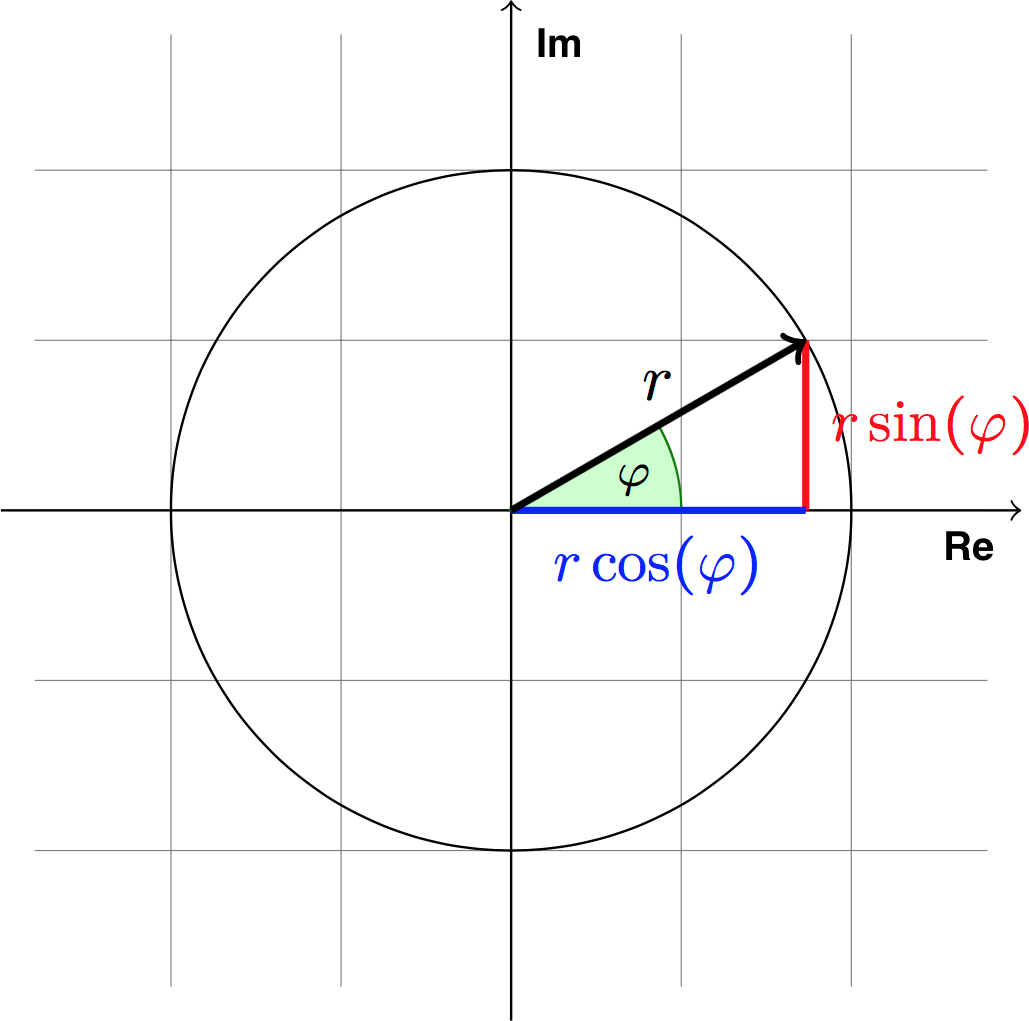
\includegraphics[width=\linewidth,keepaspectratio=true]{images/polarform}
\end{minipage}
%
\begin{minipage}[c]{0.5\textwidth}
	\begin{equation*}
	\begin{split}
	z & = x + iy = r(\cos(\varphi) + i\sin(\varphi)) = re^{i\varphi} \\
	r & = |z| = \sqrt{x^2 + y^2} \\
	\arg(z) & = \varphi  = \arctan(\frac{y}{x}) \quad \text{(je nach Quadrant)}  \\
	x & = r\cos(\varphi) \\
	y & = r\sin(\varphi) \\
	zw & = (re^{i\varphi})\cdot(se^{i\psi}) = rse^{i(\varphi + \psi)} \\
	\sqrt[q]{z} & = \sqrt[q]{s}e^{i\phi}\text{, wobei }\phi = \frac{\varphi}{q} \mod \frac{2\pi}{q} \\
	e^{i(\frac{\pi}{2} + 2\pi k)} & = i,\ e^{i\pi} = 1, \ e^{-i\pi} = -1
	\end{split}
	\end{equation*}
\end{minipage}

\begin{minipage}[c]{0.5\textwidth}
	\begin{equation*}
	\begin{split}
	(a,b) \cdot (c, d) & = (ac-bd, ad+bc) \\
	\overline{z} & = x - iy\\
	z^{-1} & = \frac{\overline{z}}{|z|^2} \\
	i & = \sqrt{-1}\\
	\end{split}
	\end{equation*}
\end{minipage}
%
\begin{minipage}[c]{0.5\textwidth}
	\begin{equation*}
	\begin{split}
	i^2 & = -1 \\
	|z|^2 & = z\overline{z} \\
	|zw|^2 & = (zw) \cdot \overline{(zw)} = |z|^2|w|^2
	\end{split}
	\end{equation*}
\end{minipage}
\figurename


\part{Tables}
\subsection{Elementare Integrale}

\begin{table}[H]
	\centering
	\begin{tabular}{|c|c|c|}
		\hline
		$f'(x)$ & $f(x)$ & $F(x)$ \\ \specialrule{.1em}{0em}{0em} 
		$\frac{f'(x)g(x) - f(x)g'(x)}{g(x)^2}$ & $\frac{f(x)}{g(x)}$ &  \\ \hline
		$0$ & $c$ & $cx$ \\ \hline
		$r\cdot x^{r-1}$ & $x^r$ & $\frac{x^{r+1}}{r+1}$ \\ \hline
		$-\frac{1}{x^2} = -x^{-2}$ & $\frac{1}{x} = x^{-1}$ & $\ln|x|$ \\ \hline
		$\frac{1}{2\sqrt{x}} = \frac{1}{2}x^{-\frac{1}{2}}$ & $\sqrt{x} = x^{\frac{1}{2}}$ & $\frac{2}{3}x^\frac{3}{2}$ \\ \hline
		$\cos(x)$ & $\sin(x)$ & $-\cos(x)$ \\ \hline
		$-\sin(x)$ & $\cos(x)$ & $\sin(x)$ \\ \hline
		$1 + \tan^2(x) = \frac{1}{\cos^2(x)}$ & $\tan(x)$ & $-\ln|\cos(x)|$ \\ \hline
		$e^x$ & $e^x$ & $e^x$ \\ \hline
		$c\cdot e^{cx}$ & $e^{cx}$ & $\frac{1}{c}\cdot e^{cx}$ \\ \hline
		$\ln(c)\cdot c^x$ & $c^x$ & $\frac{c^x}{\ln(c)}$ \\ \hline
		$\frac{1}{x}$ & $\ln|x|$ & $x(\ln|x| - 1)$ \\ \hline
		$\frac{1}{\ln(a) \cdot x}$ & $\log_a|x|$ & $\frac{x}{\ln(a)}(\ln|x| -1)$ \\ \hline
		$\frac{1}{\sqrt{1-x^2}}$ & $\arcsin(x)$ & $x\cdot\arcsin(x) + \sqrt{1-x^2}$ \\ \hline
		$-\frac{1}{\sqrt{1-x^2}}$ & $\arccos(x)$ & $x\cdot\arccos(x) - \sqrt{1-x^2}$ \\ \hline
		$\frac{1}{1+x^2}$ & $\arctan(x)$ & $x\cdot \arctan(x) - \frac{1}{2}\ln(1+x^2)$ \\ \hline
		$\cosh(x)$ & $\sinh(x) = \frac{e^x - e^{-x}}{2}$ & $\cosh(x)$ \\ \hline
		$\sinh(x)$ & $\cosh(x) = \frac{e^x + e^{-x}}{2}$ & $\sinh(x)$ \\ \hline
		$\frac{1}{\cosh^2(x)}$ & $\tanh(x)$ & $\log(\cosh(x))$ \\ \hline
	\end{tabular}
\end{table}



\subsection{Wichtige Grenzwerte}

\begin{equation*}
\begin{split}
\lim\limits_{n \to \infty} \left( 1+\frac{x}{n} \right)^n = e^x \qquad & \qquad \lim\limits_{n \to \infty} \left( 1+\frac{1}{n} \right)^n = e \\
\lim\limits_{x \to 0} \frac{a^x-1}{x} = \ln a \qquad & \qquad \lim\limits_{x \to 0} \frac{\log_a(1+x)}{x} = \frac{1}{\ln a} \\
\lim\limits_{x \to 0} \frac{1-\cos(x)}{x} = 0 \quad \qquad & \qquad \lim\limits_{x \to 0} \frac{1-\cos(x)}{x^2} = \frac{1}{2} \\
\lim\limits_{x \to 0} \frac{\tan(x)}{x} = 1 \qquad & \qquad \lim\limits_{x \to 0} \frac{\sin(x)}{x} = 1 \\
\lim\limits_{n \to \infty} \frac{n!}{n^n} = 0 \qquad & \qquad \lim\limits_{n \to 0} \frac{e^n -1 }{n} = 1 \\
\lim\limits_{n \to \infty} \sqrt[n]{n!} = \infty \qquad & \qquad \lim\limits_{n \to \infty} \sqrt[n]{n} = 1 \\
\lim\limits_{n \to \infty} \ln(n) = \infty \qquad & \qquad \lim\limits_{x \to 0} \frac{\log_a(1+x)}{x} = \frac{1}{\ln a} \\
\end{split}
\end{equation*}

\section{Formeltafel}
\subsection{Mitternachtsformel}
\[ a x + b x + c = 0 \qquad \implies \qquad x_{1,2} = \frac{-b \pm \sqrt{b^2-4ac}}{2a} \]

\subsection{Binomialkoeffizient}
\[ \binom nk = \frac{n!}{k!\,(n-k)!} \quad \mbox{für }\ 0\leq k\leq n \]

\subsection{Argument}
\[
\arg(x,y) := \begin{cases}
\arctan(\frac{y}{x}) & x \geq 0 \\
-\arctan(\frac{y}{x}) & x < 0 \\
\frac{\pi}{2} & x=0, y < 0 \\
\frac{3\pi}{2} & x = 0, y > 0
\end{cases}
\]

\subsection{Kreisfunktionen}
{\footnotesize
	\begin{tabular}{|l||c|c|c|c|c|c|c||c|c|}\hline
		$\alpha$ & $0$ & $\frac{\pi}{6}$ & $\frac{\pi}{4}$ &
		$\frac{\pi}{3}$ & $\frac{\pi}{2}$ & $\frac{2\pi}{3}$ & $\pi$ &
		Periode &Wertebereich\\
		
		& $0^\circ$ & $30^\circ$ & $45^\circ$ & $60^\circ$ & $90^\circ$ & $120^\circ$ &
		$180^\circ$ & &\\ \hline
		
		$\sin$ & $0$ & $\frac{1}{2}$ & $\frac{\sqrt{2}}{2}$ &
		$\frac{\sqrt{3}}{2}$ & $1$ & $\frac{\sqrt{3}}{2}$ & $0$ & $\sin(\alpha +
		k\cdot${$2\pi$}$)$ & $[-1,1]$\\ \hline
		
		$\cos$ & $1$ & $\frac{\sqrt{3}}{2}$ & $\frac{\sqrt{2}}{2}$ & $\frac{1}{2}$ & $0$
		& $-\frac{1}{2}$ & $-1$ & $\cos(\alpha + k\cdot${$2\pi$}$)$ & $[-1,1]$\\
		\hline
		
		
		$\tan$ & $0$ & $\frac{\sqrt{3}}{3}$ & $1$ & $\sqrt{3}$ & $\pm \infty$ &
		$-\sqrt{3}$ & $0$ & $\tan(\alpha + k \cdot${$\pi$}$)$ & $]-\infty, \infty[$
		\\
		\hline
	\end{tabular}
}



\subsection{Ableitungen}
\subsubsection{Regeln}
\begin{itemize}[leftmargin=*]
	\item (Summenregel) $(f + g)'(x) = f'(x) + g'(x)$
	\item (Produktregel) $(fg)'(x) = f'(x)g(x) + f(x)g'(x)$
	\item (Quotientenregel) $(\frac{f}{g})'(x) = \frac{f'(x)g(x) -
		f(x)g'(x)}{g^2(x)}$
	\item (Kettenregel) $(g \circ f)'(x) = (g(f(x)))' = g'(f(x)) f'(x)$
\end{itemize}

\subsubsection{Ableitungs-Tafel}
\begin{itemize}[leftmargin=*]
	\item $\frac{d}{dx}\; x^n = nx^{n-1}$
	\item $\frac{d}{dx}\; \frac{1}{x^n} = -n \frac{1}{x^{n+1}}$
	\item $\frac{d}{dx}\; \sqrt[n]{x} = \frac{1}{n\sqrt[n]{x^{n-1}}}$
	\item $\frac{d}{dx}\; e^{\alpha x + \beta} = \alpha e^{\alpha x + \beta}$
	\item $\frac{d}{dx}\; e^{x^\alpha} = \alpha x^{\alpha - 1} e^{x^\alpha}$
	\item $\frac{d}{dx}\; \ln(x) = \frac{1}{x}$
	\item $\frac{d}{dx}\; \alpha^x = \alpha^x \ln(\alpha)$
	\item $\frac{d}{dx}\; x^x = x^x (1 + \ln(x))$
	\item $\frac{d}{dx}\; x^{x^\alpha} = x^{x^\alpha + \alpha - 1} (\alpha
	\log(x) + 1)$
	\newline
	\item $\frac{d}{dx}\; \sin(x) = \cos(x)$;
	$\frac{d}{dx}\; \sin(\alpha x + \beta) = \alpha \cos(\alpha x +
	\beta)$
	\item $\frac{d}{dx}\; \cos(x) = -\sin(x)$;
	$\frac{d}{dx}\; \cos(\alpha x + \beta) = -\alpha \sin(\alpha x + \beta)$
	\item $\frac{d}{dx}\; \tan(x) = \frac{1}{cos^2(x)}$;
	$\frac{d}{dx}\; \tan(\alpha x + \beta) = \alpha \frac{1}{\cos^2(\alpha x
		+ \beta)}$
	\item $\frac{d}{dx}\; \arcsin(x) = \frac{1}{\sqrt{1-x^2}}$;  
	$\frac{d}{dx}\; \arcsin(\alpha x + \beta) =
	\frac{\alpha}{\sqrt{1-(\alpha x + \beta)^2}}$
	\item $\frac{d}{dx}\; \arccos(x) = -\frac{1}{\sqrt{1-x^2}}$;
	$\frac{d}{dx}\; \arccos(\alpha x + \beta) = -\frac{\alpha}{\sqrt{1 -
			(\alpha x + \beta)^2}}$
	\item $\frac{d}{dx}\; \arctan(x) = \frac{1}{x^2+1}$; 
	$\frac{d}{dx}\; \arctan(\alpha x + \beta) = \frac{\alpha}{(\alpha x +
		\beta)^2 + 1}$
	\newline
	\item $\frac{d}{dx}\; \sinh(x) = \cosh(x)$;
	$\frac{d}{dx}\; \sinh(\alpha x + \beta) = \alpha \cosh(\alpha x + \beta)$
	\item $\frac{d}{dx}\; \cosh(x) = \sinh(x)$;
	$\frac{d}{dx}\; \cosh(\alpha x + \beta) = \alpha \sinh(\alpha x + \beta)$
	\item $\frac{d}{dx}\; \tanh(x) = \frac{1}{\cosh^2(x)}$;
	$\frac{d}{dx}\; \tanh(\alpha x + \beta) = \alpha
	\frac{1}{\cosh^2(\alpha x + \beta)}$
	\item $\frac{d}{dx}\; arcsinh(x) = \frac{1}{\sqrt{x^2 + 1}}$;
	$\frac{d}{dx}\; arcsinh(\alpha x + \beta) = \frac{\alpha}{\sqrt{(\alpha x
			+ \beta)^2 + 1}}$
	\item $\frac{d}{dx}\; arcosh(x) = \frac{1}{\sqrt{x-1} \sqrt{x + 1}}$;
	$\frac{d}{dx}\; arcosh(\alpha x + \beta) = \frac{\alpha}{\sqrt{\alpha x + \beta
			- 1} \sqrt{\alpha x + \beta + 1}}$
	\item $\frac{d}{dx}\; arctanh(x) = \frac{1}{1-x^2}$;
	$\frac{d}{dx}\; arctanh(\alpha x + \beta) = \frac{\alpha}{1 - (\alpha x +
		\beta)^2}$
\end{itemize}

\subsection{Integrale}
\subsubsection*{Integralregeln}
Es gelte: $\int f(x) \, dx = F(x)$
\begin{itemize}[leftmargin=*]
	\item $\int u'\cdot v dx = uv - \int u \cdot v' dx$
	\item $\int f(x) dx = \int f(g(t)) \cdot g'(t) dt, \; x=g(t), dx = g'(t) dt$\newline\hfill
	\item $\int f(a + x) \,dx = F(a + x)$
	\item $\int f(a - x) \,dx = -F(a-x)$
	\item $\int f(-x) \,dx = -F(-x)$
	\item $\int f(\alpha x) \,dx = \frac{1}{\alpha}F(\alpha x)$
	\item $\int \frac{g'(x)}{g(x)} \, dx = \ln|g(x)|$
	\item $\int g(x)g'(x) \, dx = \frac{1}{2}g(x)^2$\\
	\item $|\int f(x)| \leq \int |f(x)|$ (wenn f, Riemann-Integrable ist)
\end{itemize}
\subsubsection*{typische Integrale}
\begin{itemize}[leftmargin=*]
	\item $\int \frac{1}{x} \,dx = \ln |x|$
	\item $\int \frac{1}{x^2} \,dx = -\frac{1}{x}$
	\item $\int \frac{1}{x+a} \,dx = \ln |x+a|$
	\item $\int \ln(x) \,dx = x(\ln(x) - 1)$
	\item $\int \ln(ax + b) \,dx = \frac{(a x+b) \ln (a x+b)-a x}{a}$
	\item $\int \frac{1}{(x+a)^2} \,dx = - \frac{1}{x+a}$
	\item $\int \frac{1}{\sqrt{x}} \,dx = 2 \sqrt{x}$
	\item $\int \frac{1}{ax+b} \,dx = \frac{1}{a} \ln |ax+b|$
	\item $\int \frac{1}{1 + x^2} \,dx = \frac{1}{2} \ln |1 + x^2|$
	\item $\int(ax + b)^n \,dx = \frac{(ax + b)^{n+1}}{(n + 1)a}, (n \neq -1)$
	\item $\int x(ax+b)^n \,dx = \frac{(ax + b)^{n+2}}{(n+2)a^2} -
	\frac{b(ax+b)^{n+1}}{(n+1)a^2}$
	\item $\int \frac{ax + b}{px + q} \,dx = \frac{ax}{p} + \frac{bp - aq}{p^2} \ln
	|pq+q|$
	\item $\int \frac{1}{a^2 + x^2} \,dx = \frac{1}{a} \arctan(\frac{x}{a})$
	\item $\int \frac{1}{a^2 - x^2} \,dx = \frac{1}{2a} \ln \left | \frac{a+x}{a-x}
	\right |$
	\item $\int \sqrt{x} \,dx = \frac{2}{3}\sqrt{x^3}$
	%mühsamer kerl der teilweise in prüfungen verwendet wird. Kann man über subsitution von x mit sin(u) lösen.
	\item $\int \sqrt{1-x^2} \,dx = \frac{1}{2}\left( x\sqrt{1-x^2}+\frac{1}{\sin(x)} \right)$
	\item $\int a^{xb + c} \,dx = \frac{a^{bx + c}}{b \log(a)}$
\end{itemize}

\subsubsection*{trionometrische Funktionen}
\begin{itemize}[leftmargin=*]
	\item $\int \sin(ax) \,dx = -\frac{1}{a}\cos(ax)$
	\item $\int \cos(ax) \,dx = \frac{1}{a}\sin(ax)$
	\item $\int \sin(ax)^2 \,dx = \frac{x}{2} - \frac{sin(2ax)}{4a}$
	\item $\int \frac{1}{\sin^2 x} \,dx = -\cot x$
	\item $\int x \sin(ax) \,dx = \frac{\sin(ax)}{a^2} - \frac{x \cos(ax)}{a}$
	\item $\int \cos^2(ax) \,dx = \frac{x}{2} + \frac{\sin(2ax)}{4a}$
	\item $\int \frac{1}{\cos^2(x)} \,dx = \tan x$
	\item $\int \cos(ax) \,dx = \frac{\cos(ax)}{a^2} + \frac{x \sin(ax)}{a}$
	\item $\int \sin(ax) \cos(ax) \,dx = -\frac{\cos^2(ax)}{2a}$
	\item $\int \tan(ax) \,dx = - \frac{1}{a} \ln | \cos(ax) |$
	\item $\int \arcsin(x) \,dx = x \arcsin(x) + \sqrt{1 - x^2}$
	\item $\int \arccos(x) \,dx = x \arccos(x) - \sqrt(1-x^2)$
	\item $\int \arctan(x) \,dx = x \arctan(x) - \frac{1}{2} \ln(1+x^2)$
\end{itemize}

\subsubsection*{Hyperbelfunktionen}
\begin{itemize}[leftmargin=*]
	\item $\int \sinh(ax + b) \,dx = \frac{\cosh(ax + b)}{a}$; $\int \sinh(x) \,dx
	= \cosh(x)$
	\item $\int \cosh(ax + b) \,dx = \frac{\sinh(ax + b)}{a}$; $\int \cosh(x) \,dx
	= \sinh(x)$
	\item $\int \tan(ax + b) \,dx = \frac{\log(\cosh(ax+b))}{a}$; $\int \tan(x)
	\,dx = \log(\cosh(x))$
\end{itemize}

\subsubsection*{Exponentialfunktion}
\begin{itemize}[leftmargin=*]
	\item $\int e^{ax} \,dx = \frac{1}{a} e^{ax}$ 
	\item $\int x e^{ax} \,dx = e^{ax} \cdot \left ( \frac{ax - 1}{a^2} \right )$
	\item $\int x \ln(x) \,dx = \frac{1}{2} x^2 (\ln(x) - \frac{1}{2})$
	\item $\int_{-\infty}^\infty e^{-\frac{1}{a}x^2} \,dx = \sqrt{a \pi}$
\end{itemize}

\subsection{Reihen}
\begin{itemize}[leftmargin=*]
	\item $\sum_{n=1}^\infty \frac{1}{n}$ divergiert (``harmonische Reihe'')
	\item $\sum_{n=1}^\infty \frac{(-1)^n}{n} = \ln \frac{1}{2}$
	\item $\sum_{n=1}^\infty \frac{1}{n^\alpha}$ konvergiert für $\alpha > 1$,
	divergiert für $\alpha \leq 1$
	\item $\sum_{n=0}^\infty q^n = \frac{1}{1-q}$ für $|q| < 1$ (``geometrische
	Reihe'')
	\item $\sum_{n=0}^\infty (-1)^n q^n = \frac{1}{1-q}$ für $|q| < 1$ (``geometrische
	Reihe'')
	\item $\sum_{n=1}^\infty \frac{1}{n^2} = \frac{\pi^2}{6}$
	\newline
	\item $\sum_{n=1}^m n = \frac{m(m+1)}{2}$
	\item $\sum_{n=0}^m q^n = \frac{1-q^{m+1}}{1-q}$ 
	\item  $\sum_{n=0}^m n^2 = \frac{1}{6}m(m+1)(2m+1)$
	\item  $\sum_{n=0}^m n^3 = \frac{1}{4}m^2(m+1)^2$
\end{itemize}

\subsection{Reihenentwicklung}
\begin{itemize}[leftmargin=*]
	\item $e^x = \sum_{n=0}^\infty \frac{x^n}{n!} = 1 + \frac{x}{1!} +
	\frac{x^2}{2!} + \cdots$
	\item $\ln(1 + x) = \sum_{n=1}^\infty  (-1)^{(n+1)} \frac{x^n}{n} $
	\item $-\ln(1 - x) = \sum_{n=1}^\infty  \frac{x^n}{n} $
	\item $\ln x = \sum_{n=0}^\infty \frac{2}{2n + 1} \cdot \left(
	\frac{x-1}{x+1} \right)^{2n}$
	
	\item $\frac{1}{1-x} = \sum_{n=0}^\infty x^{n}$ für $|x|<1$ (Geom. Reihe)
	\item $\frac{1}{(1-x)^2} = \sum_{n=0}^\infty nx^{(n-1)}$
	
	\item $\sin x = \sum_{n=0}^\infty (-1)^n \frac{x^{2n + 1}}{(2n + 1)!} = x -
	\frac{x^3}{3!} + \frac{x^5}{5!} + \cdots$
	\item $\cos x = \sum_{n=0}^\infty (-1)^n \frac{x^{2n}}{(2n)!} = 1 -
	\frac{x^2}{2!} + \frac{x^4}{4!} - \cdots + \cdots$
	\item $\sinh x = \sum_{n=0}^\infty \frac{x^{2n+1}}{(2n + 1)!}$
	\item $\cosh x = \sum_{n=0}^\infty \frac{x^{2n}}{(2n)!}$
	\item $\arcsin x =  \sum_{k=0}^{\infty} \binom{2k}{k} \frac{x^{2k+1}}{4^{k}(2k+1)}$
	\item $\arccos x = \frac{\pi}{2} - \arcsin x$
	\item $\arctan x = \sum_{n=0}^\infty (-1)^n \frac{x^{(2n+1)}}{2n+1}$ für $|x|<1$
\end{itemize}

\subsection{Grenzwerte}
\begin{itemize}[leftmargin=*]
	\item \textbf{Bernoullische Ungleichung}: $x \geq -1, n \in \N: \; (1+x)^n \geq
	1+nx$
	\item \textbf{Vergleich von Folgen}: weiter rechts stehende Folgen streben
	schneller gegen $\infty$ als die links davon stehenden:\\ $1, \quad \ln n, \quad
	n^\alpha (\alpha > 0), \quad q^n (q > 1), \quad n!, \quad n^n$ $\Rightarrow
	\lim_{x \to \infty} \frac{\ln n}{n^\alpha} = 0$
\end{itemize}
\subsubsection*{$\lim_{n \to \infty}$}
\begin{itemize}[leftmargin=*]
	\item $\lim_{n \to \infty} \sqrt[n]{a} \rightarrow 1$
	\item $\lim_{n \to \infty} \sqrt[n]{n} \rightarrow 1$
	\item $\lim_{n \to \infty} \sqrt[n]{n!} \rightarrow \infty$
	\item $\lim_{n \to \infty} \frac{n}{\sqrt[n]{n!}} \rightarrow e$
	\item $\lim_{n \to \infty} \frac{1}{n} \sqrt[n]{n!} \rightarrow \frac{1}{e}$
	\item $\lim_{n \to \infty} \left ( \frac{n+1}{n} \right )^n \rightarrow e$
	\item $\lim_{n \to \infty} \left ( 1 + \frac{1}{n} \right )^n \rightarrow e$
	\item $\lim_{n \to \infty} \left ( 1 - \frac{1}{n} \right )^n \rightarrow \frac{1}{e}$
	\item $\lim_{n \to \infty} \left ( 1 + \frac{x}{n} \right )^n \rightarrow e^x$
	\item $\lim_{n \to \infty} \left ( 1 - \frac{x}{n} \right )^n \rightarrow \frac{1}{e^x}$
	\item $\lim_{n \to \infty} {a \choose n} \rightarrow 0, \; a > -1$
	\item $\lim_{n \to \infty} \frac{a^n}{n!} \rightarrow 0$
	\item $\lim_{n \to \infty} \frac{n^n}{n!} \rightarrow \infty$
	\item $\lim_{n \to \infty} \frac{a^n}{n^k} \rightarrow \infty, a > 1, k$ fest
	\item $\lim_{n \to \infty} a^n n^k \rightarrow 0, |a| < 1, k$ fest
	\item $\lim_{n \to \infty} n(\sqrt[n]{a} - 1) \rightarrow \ln a, a > 0$
	\item $\lim_{n \to \infty} \left( 1+\frac{x}{n} \right)^n = e^x \quad$
	\item $\lim_{n \to \infty} \sqrt[n]{n} = 1$
	\item $\lim_{n \to \infty} n^p q^n = 0 \qquad p \in \N \text{ und } 0 < q < 1$
	\item $\lim_{x \to \infty} \sqrt{x^2-x}-x = \frac{1}{2}$ \newline{\small (Lösungsansatz mit Taylorreihe
		($\sqrt{1-x} = 1 + \frac{x}{2}+O(x^2)$): $\sqrt{x^2-x}-x = x(\sqrt{1-\frac{1}{x}}-1) =
		x((1+\frac{1}{2x}+O(\frac{1}{x^2}))-1) = \frac{1}{2}+O(\frac{1}{x}) \underset{n \to \infty}{\longrightarrow} \frac{1}{2}$ )}
\end{itemize}
\subsubsection*{$\lim_{x \to 0}$}
\begin{itemize}[leftmargin=*]
	\item $\lim_{x \to 0} \frac{a^x - 1}{x} = \ln a$
	\item $\lim_{x \to 0} \frac{\sin x}{x} = 1$
	\item $\lim_{x \to 0} \frac{1 - \cos x}{x} = 0$
	\item $\lim_{x \to 0} \frac{\log_a (1 + x)}{x} = \frac{1}{\ln a}$
	\item $\lim_{x \to 0} x^a \ln x = 0, \; a  > 0$
	\item $\lim_{x \to 0} \frac{a^x-1}{x} = \ln a$ 
	\item $\lim_{x \to 0} \frac{\sin(x)}{x} = 1$ 
	\item $\lim_{x \to 0} \frac{1-\cos(x)}{x} = 0 \quad$ 
	\item $\lim_{x \to 0} \frac{\log_a(1+x)}{x} = \frac{1}{\ln a}$
	\item $\lim_{x \to 0} x^\alpha \ln x = 0 \qquad \alpha > 0$
\end{itemize}

\subsection{Linienintegral}
\begin{itemize}[leftmargin=*]
	\item 2. Art: $\int_\gamma \vec{f}(\vec{x}) d\vec{x} := \int_a^b \left<
	\vec{f}(\gamma(t)), \gamma(t)' \right>\; dt$
	\item 1. Art: $\int_\gamma f ds := \int_a^b f(\gamma(t)) \|\gamma(t)'\|_2\; dt$
\end{itemize}

\subsection{Kreuzprodukt}
{\footnotesize
	\[
	\vec{a} \times \vec{b} = \left ( \begin{array}{c} a_1 \\ a_2 \\ a_3 \end{array}
	\right ) \times
	\left ( \begin{array}{c} b_1 \\ b_2 \\ b_3 \end{array}
	\right ) =
	\left ( \begin{array}{c} a_2b_3 - a_3b_2 \\ a_3b_1 - a_1b_3 \\ a_1b_2 - a_2b_1
	\end{array} \right )
	\]
}


\subsection{Exponent}
\begin{itemize}[leftmargin=*]
	\item $a^n a^m = a^{n + m}$
	\item $(a^n)^m = a^{nm}$
	\item $(ab)^n = a^n b^n$
	\item $\left( \frac{a}{b} \right)^n = \frac{a^n}{b^n}$
	\item $a^{-n} = \frac{1}{a^n}$
	\item $\left( \frac{a}{b} \right)^{-n} = \left( \frac{b}{a} \right)^n$
	\item $a^\frac{n}{m} = (a^\frac{1}{m})^n = (a^n)^\frac{1}{m}$
\end{itemize}


\subsection{Wurzel}
\begin{itemize}[leftmargin=*]
	\item $\sqrt[n]{a} = a^\frac{1}{n}$
	\item $\sqrt[n]{ab} = \sqrt[n]{a} \sqrt[n]{b}$
	\item $\sqrt[m]{\sqrt[n]{a}} = \sqrt[nm]{a}$
	\item $\sqrt[n]{\frac{a}{b}} = \frac{\sqrt[n]{a}}{\sqrt[n]{b}}$
\end{itemize}



\subsection{Ungleichungen}
\begin{itemize}[leftmargin=*]
	\item $a < b \Rightarrow a + c < b + c$ und $a - c < b - c$
	\item $a < b$ und $c > 0 \Rightarrow \frac{a}{c} < \frac{b}{c}$
	\item $a < b$ und $c < 0 \Rightarrow \frac{a}{c} > \frac{b}{c}$ 
	\item Dreiecksungleichung für reelle Zahlen: $|a+b| \le |a|{+}|b|$ %Quelle Wikipedia: http://de.wikipedia.org/wiki/Dreiecksungleichung#Dreiecksungleichung_f.C3.BCr_reelle_Zahlen
	\item Cauchy-Schwarz Ungleichung: $|x \cdot y| \leq \|x\| \cdot \|y\|, \; x,y \in \R^n$
\end{itemize}

\subsection{Logarithmen}
\begin{itemize}[leftmargin=*]
	\item $e^{-\infty} = 0$
	\item $e^0 = 1$
	\item $e^1 = e =  2.718281828$
	\item $e^{\infty} = \infty$
\end{itemize}

\begin{itemize}[leftmargin=*]
	\item $y = \log_a x \Leftrightarrow x = a^y$
	\item $\log_a 1 = 0$
	\item $\log_a a^x = x$
	\item $a^{\log_a x} = x $
	\item $\log_a xy = \log_a x + \log_a y$
	\item $\log_a \frac{1}{x} = - \log_a x$
	\item $\log_a x^r = r \log_a x$
	\item $\log_a x = \frac{\log_b x}{\log_b a}$
	\item $\log_a x = \frac{\ln x}{\ln a}$
	\item $\log_a (x+y) = \log_a x + log_a (1 + \frac{y}{x})$
	\item $\log_a (x-y) = \log_a x + \log_a (1- \frac{y}{x})$
	\item $e^{a+bi} = e^a(\cos(b) + i \sin(b))$ (Euler Identität)
	\item $e^{b \ln(a)} = a^b$
	\item $ e^{-\ln(b)} = \frac{1}{b}$
\end{itemize}

\subsection{Komplexe Zahlen}
\begin{itemize}[leftmargin=*]
	\item $z \in \C: z = a + b\cdot i$
	\item $\bar{z} = a - b\cdot i$
	\item $|z|^2 = z \cdot \bar{z} = (a + b\cdot i) \cdot (a - b\cdot i) = a^2 + b^2$
	\item $i^2 = -1$
	\item $(a + bi) + (c + di) = (a + c) + (b + d)i$
	\item $(a + bi) \cdot (c + di) = (ac - bd) + (ad + bc)i$
	\item $\frac{a + bi}{c + di} = \frac{ac + bd}{c^2 + d^2} + \frac{bc - ad}{c^2 + d^2}\cdot i$
\end{itemize}

\subsection{Geometrische Körper}
\subsubsection{Ellipsoid}
Hat die Form eines Rugbyballs. In kartesischen Koordinaten definert durch
$\frac{x^2}{a^2} + \frac{y^2}{b^2} + \frac{z^2}{c^2} - 1 = 0$.

\subsection{Geometrie in 3D}
%evtl. nicht nötig. Aber in alten prüfungen oft gefragt.
\subsubsection*{Masse von speziellen Gebieten}

\renewcommand\arraystretch{1.4}
\begin{tabular}{l|l}
	Zylinder   &   $ V = \pi r^2 h $ \\
	Pyramide   &   $ V = \frac{1}{3} G h $ \\
	Ellipsoid   &   $ V = \frac{4 \pi}{3} a b c $ \\
	Kegel   &   $ V = \frac{\pi}{3} r^2 h $ \\
	Kegelstumpf   &   $ V = \frac{\pi h}{3} (r_1^2+r_2^2 + r_1 r_2) $ \\
		Torus   &   $ V = 2 \pi^2 R r^2 $ \\
	&   $ S = 4 \pi^2 R r $ \\
	Kugel   &   $ V = \frac{4 \pi}{3} r^3 $ \\
	&   $ S = 4 \pi r^2 $ 
\end{tabular}


\subsubsection*{Rotationskörper}
Rotation um die x Achse $V=\pi \int_a^b f(x)^2 dx.$\\
Rotation um die y Achse $V=2\pi \int_a^b x \cdot f(x) dx.$



\subsection{Ausklammern}
\begin{itemize}[leftmargin=*]
	\item $x^n - y^n = (x-y) (x^{n-1} + x^{n-2}y + x^{n-3}y^2 + \ldots + xy^{n-2}
	+ y^{n-1})$
	\item $x^n - 1 = (x-1)(x^{n-1} + x^{n-2} + \ldots + x + 1)$
\end{itemize}

\subsection{Aus Serien}
\begin{itemize}[leftmargin=*]
	\item Ableitung von $x^x$ kann man berechnen, indem man $x = e^{\log(x)}$
	setzt. Also in diesem Fall $e^{\log(x^x)} = e^{x \log(x)}$ ableitet, was $e^{x
		\log(x)} (1 + \log(x))$ (Serie 10)
	\item Cauchy-Schwarz Ungleichung: $|x \cdot y| \leq \|x\| \cdot \|y\|, \; x,y \in \R^n$
	\item Euler Identität (komplexe Zahlen): $e^{ix} = \cos(x) + i \sin(x)$
\end{itemize}

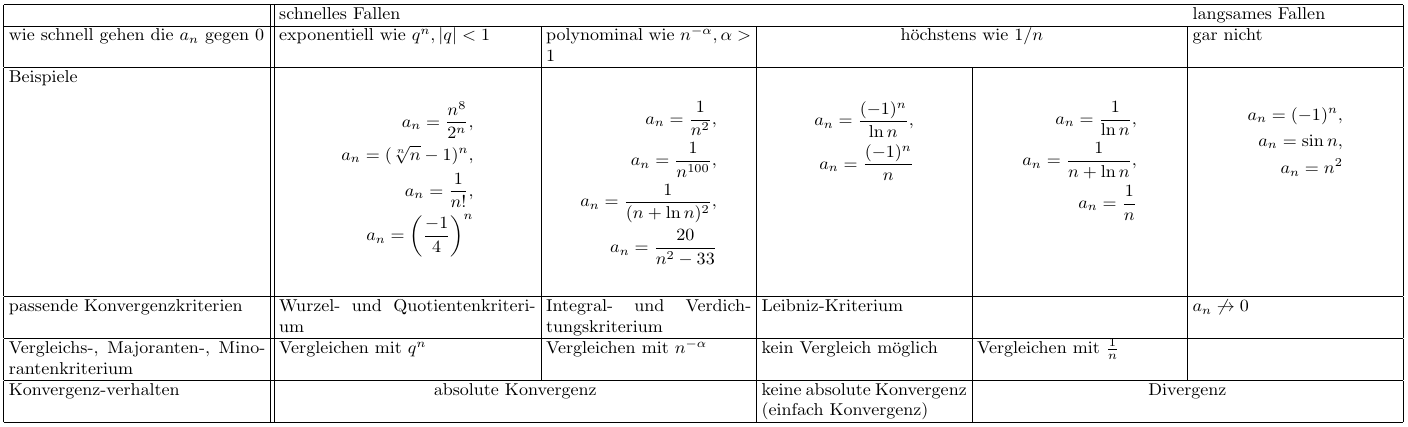
\includegraphics[width=1\textwidth]{images/Reihen_Tables.png}

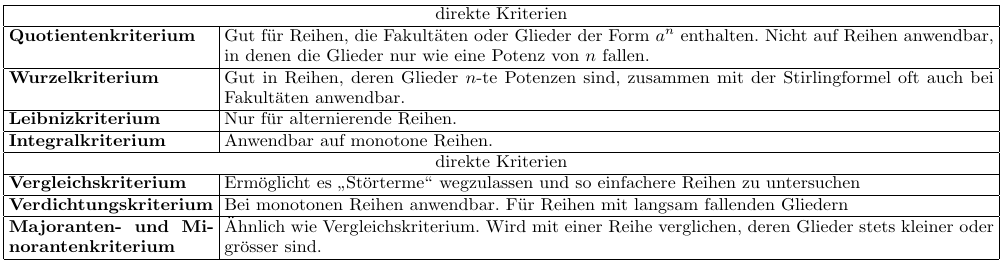
\includegraphics[width=1\textwidth]{images/Reihen_Kriterien.png}

%\part{TEMP}
%\section{Formeltafel}
\subsection{Mitternachtsformel}
\[ a x + b x + c = 0 \qquad \implies \qquad x_{1,2} = \frac{-b \pm \sqrt{b^2-4ac}}{2a} \]

\subsection{Binomialkoeffizient}
\[ \binom nk = \frac{n!}{k!\,(n-k)!} \quad \mbox{für }\ 0\leq k\leq n \]

\subsection{Argument}
\[
	\arg(x,y) := \begin{cases}
		\arctan(\frac{y}{x}) & x \geq 0 \\
		-\arctan(\frac{y}{x}) & x < 0 \\
		\frac{\pi}{2} & x=0, y < 0 \\
		\frac{3\pi}{2} & x = 0, y > 0
	\end{cases}
\]

\subsection{Kreisfunktionen}
{\footnotesize
\begin{tabular}{|l||c|c|c|c|c|c|c||c|c|}\hline
\multirow{2}{*}{$\alpha$} & $0$ & $\frac{\pi}{6}$ & $\frac{\pi}{4}$ &
$\frac{\pi}{3}$ & $\frac{\pi}{2}$ & $\frac{2\pi}{3}$ & $\pi$ &
\multirow{2}{*}{Periode} & \multirow{2}{*}{Wertebereich}\\

& $0^\circ$ & $30^\circ$ & $45^\circ$ & $60^\circ$ & $90^\circ$ & $120^\circ$ &
$180^\circ$ & &\\ \hline

$\sin$ & $0$ & $\frac{1}{2}$ & $\frac{\sqrt{2}}{2}$ &
$\frac{\sqrt{3}}{2}$ & $1$ & $\frac{\sqrt{3}}{2}$ & $0$ & $\sin(\alpha +
k\cdot$\hl{$2\pi$}$)$ & $[-1,1]$\\ \hline

$\cos$ & $1$ & $\frac{\sqrt{3}}{2}$ & $\frac{\sqrt{2}}{2}$ & $\frac{1}{2}$ & $0$
& $-\frac{1}{2}$ & $-1$ & $\cos(\alpha + k\cdot$\hl{$2\pi$}$)$ & $[-1,1]$\\
\hline


$\tan$ & $0$ & $\frac{\sqrt{3}}{3}$ & $1$ & $\sqrt{3}$ & $\pm \infty$ &
$-\sqrt{3}$ & $0$ & $\tan(\alpha + k \cdot$\hl{$\pi$}$)$ & $]-\infty, \infty[$
\\
\hline
\end{tabular}
}
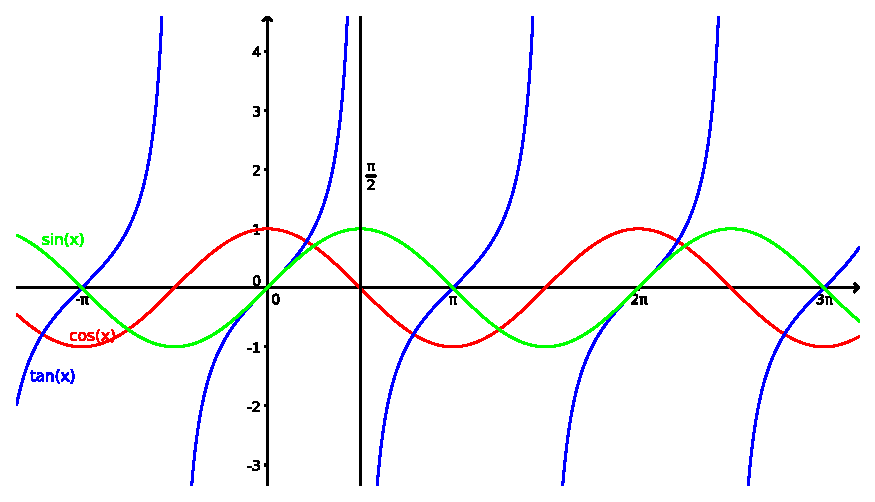
\includegraphics[width=\columnwidth]{sin_cos_tan.eps}

\subsubsection{Einheitskreis}
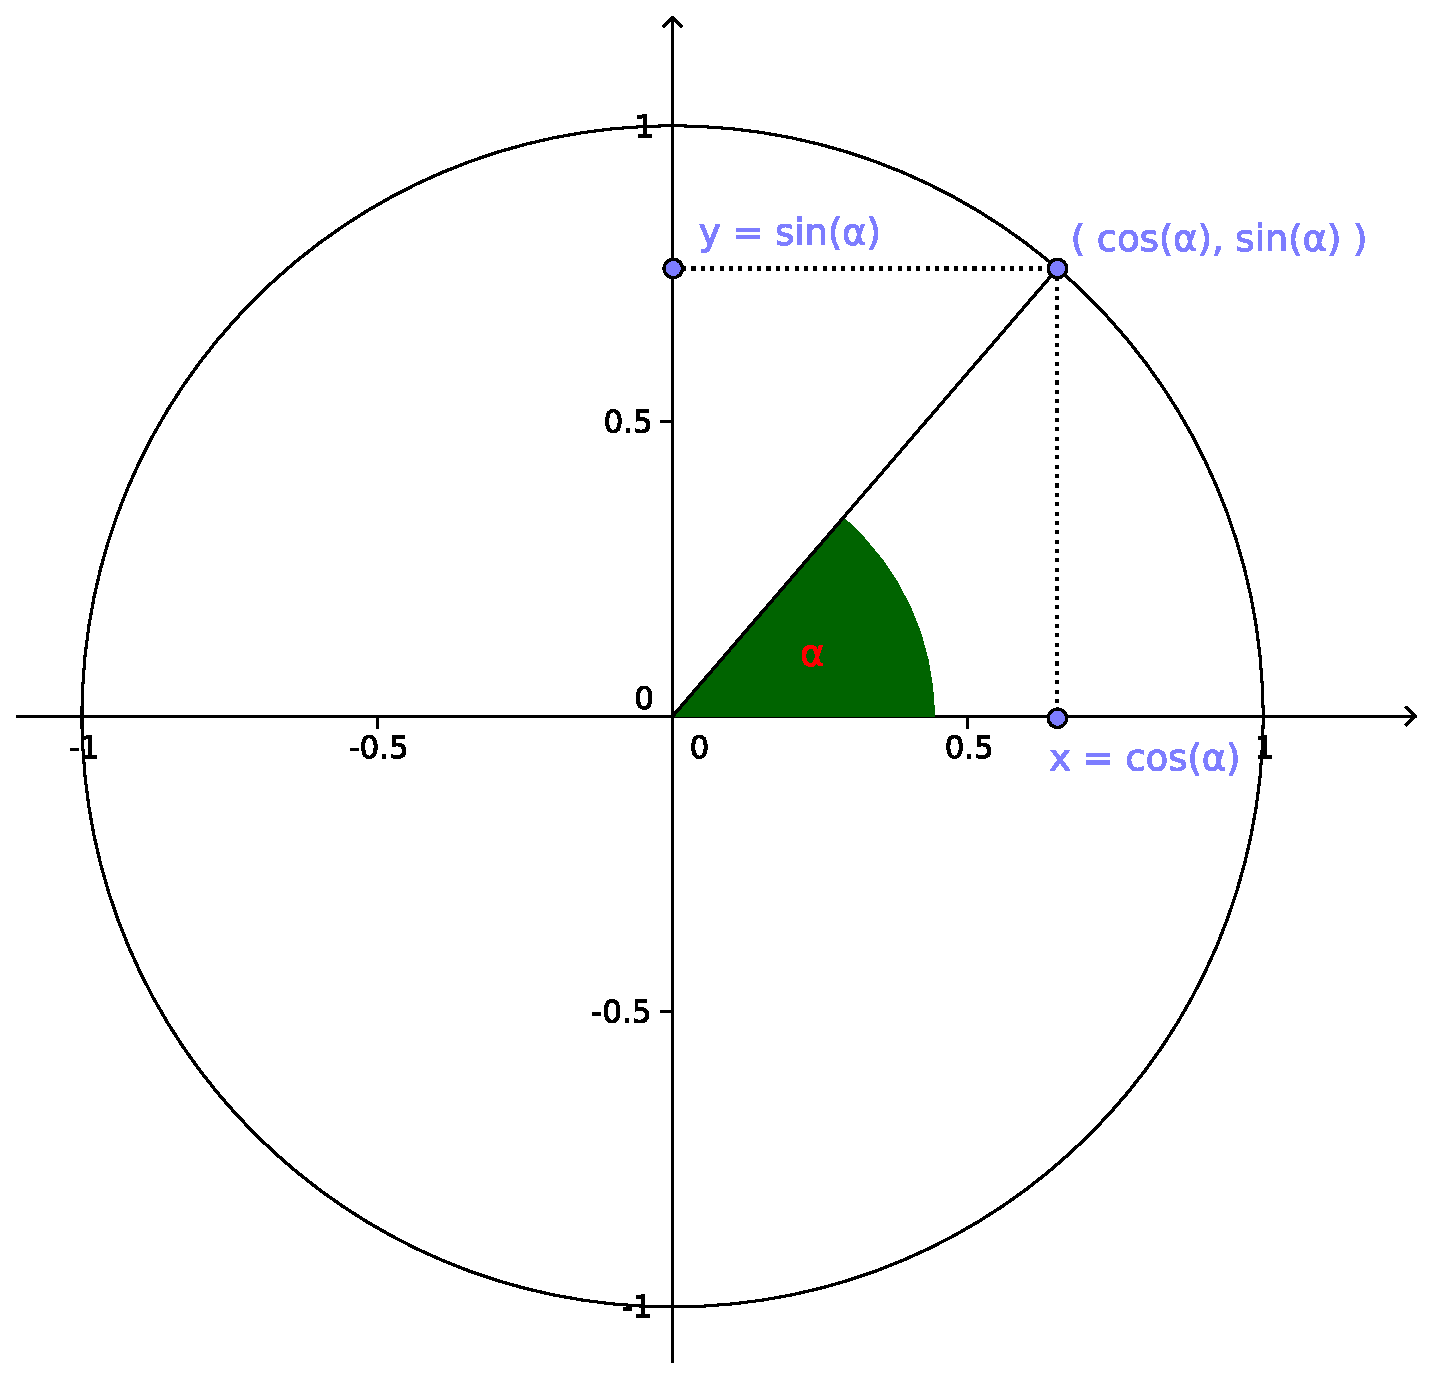
\includegraphics[width=\columnwidth]{einheitskreis_sin_cos.eps}
$\tan \alpha = \frac{\sin \alpha}{\cos \alpha} = \frac{y}{x}$

\subsection{Trigonometrische Funktionen \& Additionstheorem}
\begin{itemize}[leftmargin=*]
	\item $\sin^2(x) + \cos^2(x) = 1$
	\item $\frac{1}{\cos^2(\alpha)} = 1 + \tan^2(\alpha)$
	\item $\sin(90^\circ \pm \alpha) = \cos(\alpha)$
	\item $\sin(180^\circ \pm \alpha) = \mp \sin(\alpha)$
	\item $\cos(90^\circ \pm \alpha) = \mp \sin(\alpha)$
	\item $\cos(180^\circ \pm \alpha) = - \cos(\alpha)$
	\item $\sin(\alpha \pm \beta) = \sin(\alpha)\cos(\beta) \pm
	\cos(\alpha)\sin(\beta)$
	\item $\cos(\alpha \pm \beta) = \cos(\alpha)\cos(\beta) \mp \sin(\alpha)
	\sin(\beta)$
	\item $\tan(\alpha \pm \beta) = \frac{\tan(\alpha) \pm \tan(\beta)}{1 \mp
	\tan(\alpha)\tan(\beta)}$
	\item $\sin(2\alpha) = 2 \sin(\alpha)\cos(\alpha)$
	\item $\cos(2\alpha) = \cos^2(\alpha) - \sin^2(\alpha) = 2 \cos^2(\alpha) - 1
	= 1 - 2 \sin^2(\alpha)$
	\item $\tan(2\alpha) = \frac{2 \tan(\alpha)}{1 - \tan^2(\alpha)}$
\end{itemize}

\subsection{Hyperbelfunktionen}
\begin{itemize}[leftmargin=*]
	\item $\sinh(x) = \frac{1}{2}(e^x - e^{-x}) = -i \sin(ix)$
	\item $\cosh(x) = \frac{1}{2}(e^x + e^{-x}) = \cos(ix)$
	\item $\tanh(x) = \frac{\sinh(x)}{\cosh(x)} = \frac{e^x - e^{-x}}{e^x +
	e^{-x}} = \frac{e^{2x} - 1}{e^{2x} + 1} = 1 - \frac{2}{e^{2x} + 1}$
	\item $\arcsinh(x) = \ln(x + \sqrt{x^2 + 1})$
	\item $\arcosh(x) = \ln(x + \sqrt{x^2 - 1})$
	\item $\arctanh(x) = \frac{1}{2} \ln(\frac{1+x}{1-x})$
	\item Umformung: $\tanh(x) + 1 = \frac{e^{2x} - 1}{e^{2x} + 1} + 1 = \frac{2x -
	1 + e^{2x} + 1}{e^{2x} + 1} = \frac{2e^{2x}}{e^{2x} + 1}$
\end{itemize}


\subsection{Ableitungen}
\subsubsection{Regeln}
\begin{itemize}[leftmargin=*]
	\item (Summenregel) $(f + g)'(x) = f'(x) + g'(x)$
	\item (Produktregel) $(fg)'(x) = f'(x)g(x) + f(x)g'(x)$
	\item (Quotientenregel) $(\frac{f}{g})'(x) = \frac{f'(x)g(x) -
	f(x)g'(x)}{g^2(x)}$
	\item (Kettenregel) $(g \circ f)'(x) = (g(f(x)))' = g'(f(x)) f'(x)$
\end{itemize}

\subsubsection{Ableitungs-Tafel}
\begin{itemize}[leftmargin=*]
	\item $\frac{d}{dx}\; x^n = nx^{n-1}$
	\item $\frac{d}{dx}\; \frac{1}{x^n} = -n \frac{1}{x^{n+1}}$
	\item $\frac{d}{dx}\; \sqrt[n]{x} = \frac{1}{n\sqrt[n]{x^{n-1}}}$
	\item $\frac{d}{dx}\; e^{\alpha x + \beta} = \alpha e^{\alpha x + \beta}$
	\item $\frac{d}{dx}\; e^{x^\alpha} = \alpha x^{\alpha - 1} e^{x^\alpha}$
	\item $\frac{d}{dx}\; \ln(x) = \frac{1}{x}$
	\item $\frac{d}{dx}\; \alpha^x = \alpha^x \ln(\alpha)$
	\item $\frac{d}{dx}\; x^x = x^x (1 + \ln(x))$
	\item $\frac{d}{dx}\; x^{x^\alpha} = x^{x^\alpha + \alpha - 1} (\alpha
	\log(x) + 1)$
	\newline
	\item $\frac{d}{dx}\; \sin(x) = \cos(x)$;
	$\frac{d}{dx}\; \sin(\alpha x + \beta) = \alpha \cos(\alpha x +
	\beta)$
	\item $\frac{d}{dx}\; \cos(x) = -\sin(x)$;
	$\frac{d}{dx}\; \cos(\alpha x + \beta) = -\alpha \sin(\alpha x + \beta)$
	\item $\frac{d}{dx}\; \tan(x) = \frac{1}{cos^2(x)}$;
	$\frac{d}{dx}\; \tan(\alpha x + \beta) = \alpha \frac{1}{\cos^2(\alpha x
	+ \beta)}$
	\item $\frac{d}{dx}\; \arcsin(x) = \frac{1}{\sqrt{1-x^2}}$;  
		$\frac{d}{dx}\; \arcsin(\alpha x + \beta) =
	\frac{\alpha}{\sqrt{1-(\alpha x + \beta)^2}}$
	\item $\frac{d}{dx}\; \arccos(x) = -\frac{1}{\sqrt{1-x^2}}$;
		$\frac{d}{dx}\; \arccos(\alpha x + \beta) = -\frac{\alpha}{\sqrt{1 -
	(\alpha x + \beta)^2}}$
	\item $\frac{d}{dx}\; \arctan(x) = \frac{1}{x^2+1}$; 
		$\frac{d}{dx}\; \arctan(\alpha x + \beta) = \frac{\alpha}{(\alpha x +
	\beta)^2 + 1}$
	\newline
	\item $\frac{d}{dx}\; \sinh(x) = \cosh(x)$;
	$\frac{d}{dx}\; \sinh(\alpha x + \beta) = \alpha \cosh(\alpha x + \beta)$
	\item $\frac{d}{dx}\; \cosh(x) = \sinh(x)$;
	$\frac{d}{dx}\; \cosh(\alpha x + \beta) = \alpha \sinh(\alpha x + \beta)$
	\item $\frac{d}{dx}\; \tanh(x) = \frac{1}{\cosh^2(x)}$;
	$\frac{d}{dx}\; \tanh(\alpha x + \beta) = \alpha
	\frac{1}{\cosh^2(\alpha x + \beta)}$
	\item $\frac{d}{dx}\; \arcsinh(x) = \frac{1}{\sqrt{x^2 + 1}}$;
	$\frac{d}{dx}\; \arcsinh(\alpha x + \beta) = \frac{\alpha}{\sqrt{(\alpha x
	+ \beta)^2 + 1}}$
	\item $\frac{d}{dx}\; \arcosh(x) = \frac{1}{\sqrt{x-1} \sqrt{x + 1}}$;
	$\frac{d}{dx}\; \arcosh(\alpha x + \beta) = \frac{\alpha}{\sqrt{\alpha x + \beta
	- 1} \sqrt{\alpha x + \beta + 1}}$
	\item $\frac{d}{dx}\; \arctanh(x) = \frac{1}{1-x^2}$;
	$\frac{d}{dx}\; \arctanh(\alpha x + \beta) = \frac{\alpha}{1 - (\alpha x +
	\beta)^2}$
\end{itemize}

\subsection{Integrale}
\subsubsection*{Integralregeln}
Es gelte: $\int f(x) \, dx = F(x)$
\begin{itemize}[leftmargin=*]
	\item $\int u'\cdot v dx = uv - \int u \cdot v' dx$
	\item $\int f(x) dx = \int f(g(t)) \cdot g'(t) dt, \; x=g(t), dx = g'(t) dt$\newline\hfill
	\item $\int f(a + x) \,dx = F(a + x)$
	\item $\int f(a - x) \,dx = -F(a-x)$
	\item $\int f(-x) \,dx = -F(-x)$
	\item $\int f(\alpha x) \,dx = \frac{1}{\alpha}F(\alpha x)$
	\item $\int \frac{g'(x)}{g(x)} \, dx = \ln|g(x)|$
	\item $\int g(x)g'(x) \, dx = \frac{1}{2}g(x)^2$\\
	\item $|\int f(x)| \leq \int |f(x)|$ (wenn f, Riemann-Integrable ist)
\end{itemize}
\subsubsection*{typische Integrale}
\begin{itemize}[leftmargin=*]
  	\item $\int \frac{1}{x} \,dx = \ln |x|$
	\item $\int \frac{1}{x^2} \,dx = -\frac{1}{x}$
  	\item $\int \frac{1}{x+a} \,dx = \ln |x+a|$
  	\item $\int \ln(x) \,dx = x(\ln(x) - 1)$
  	\item $\int \ln(ax + b) \,dx = \frac{(a x+b) \ln (a x+b)-a x}{a}$
  	\item $\int \frac{1}{(x+a)^2} \,dx = - \frac{1}{x+a}$
  	\item $\int \frac{1}{\sqrt{x}} \,dx = 2 \sqrt{x}$
	\item $\int \frac{1}{ax+b} \,dx = \frac{1}{a} \ln |ax+b|$
	\item $\int \frac{1}{1 + x^2} \,dx = \frac{1}{2} \ln |1 + x^2|$
	\item $\int(ax + b)^n \,dx = \frac{(ax + b)^{n+1}}{(n + 1)a}, (n \neq -1)$
	\item $\int x(ax+b)^n \,dx = \frac{(ax + b)^{n+2}}{(n+2)a^2} -
	\frac{b(ax+b)^{n+1}}{(n+1)a^2}$
	\item $\int \frac{ax + b}{px + q} \,dx = \frac{ax}{p} + \frac{bp - aq}{p^2} \ln
	|pq+q|$
	\item $\int \frac{1}{a^2 + x^2} \,dx = \frac{1}{a} \arctan(\frac{x}{a})$
	\item $\int \frac{1}{a^2 - x^2} \,dx = \frac{1}{2a} \ln \left | \frac{a+x}{a-x}
	\right |$
	\item $\int \sqrt{x} \,dx = \frac{2}{3}\sqrt{x^3}$
	%mühsamer kerl der teilweise in prüfungen verwendet wird. Kann man über subsitution von x mit sin(u) lösen.
	\item $\int \sqrt{1-x^2} \,dx = \frac{1}{2}\left( x\sqrt{1-x^2}+\frac{1}{\sin(x)} \right)$
	\item $\int a^{xb + c} \,dx = \frac{a^{bx + c}}{b \log(a)}$
\end{itemize}

\subsubsection*{trionometrische Funktionen}
\begin{itemize}[leftmargin=*]
	\item $\int \sin(ax) \,dx = -\frac{1}{a}\cos(ax)$
	\item $\int \cos(ax) \,dx = \frac{1}{a}\sin(ax)$
	\item $\int \sin(ax)^2 \,dx = \frac{x}{2} - \frac{sin(2ax)}{4a}$
	\item $\int \frac{1}{\sin^2 x} \,dx = -\cot x$
	\item $\int x \sin(ax) \,dx = \frac{\sin(ax)}{a^2} - \frac{x \cos(ax)}{a}$
	\item $\int \cos^2(ax) \,dx = \frac{x}{2} + \frac{\sin(2ax)}{4a}$
	\item $\int \frac{1}{\cos^2(x)} \,dx = \tan x$
	\item $\int \cos(ax) \,dx = \frac{\cos(ax)}{a^2} + \frac{x \sin(ax)}{a}$
	\item $\int \sin(ax) \cos(ax) \,dx = -\frac{\cos^2(ax)}{2a}$
	\item $\int \tan(ax) \,dx = - \frac{1}{a} \ln | \cos(ax) |$
	\item $\int \arcsin(x) \,dx = x \arcsin(x) + \sqrt{1 - x^2}$
	\item $\int \arccos(x) \,dx = x \arccos(x) - \sqrt(1-x^2)$
	\item $\int \arctan(x) \,dx = x \arctan(x) - \frac{1}{2} \ln(1+x^2)$
\end{itemize}

\subsubsection*{Hyperbelfunktionen}
\begin{itemize}[leftmargin=*]
	\item $\int \sinh(ax + b) \,dx = \frac{\cosh(ax + b)}{a}$; $\int \sinh(x) \,dx
	= \cosh(x)$
	\item $\int \cosh(ax + b) \,dx = \frac{\sinh(ax + b)}{a}$; $\int \cosh(x) \,dx
	= \sinh(x)$
	\item $\int \tan(ax + b) \,dx = \frac{\log(\cosh(ax+b))}{a}$; $\int \tan(x)
	\,dx = \log(\cosh(x))$
\end{itemize}

\subsubsection*{Exponentialfunktion}
\begin{itemize}[leftmargin=*]
  	\item $\int e^{ax} \,dx = \frac{1}{a} e^{ax}$ 
	\item $\int x e^{ax} \,dx = e^{ax} \cdot \left ( \frac{ax - 1}{a^2} \right )$
	\item $\int x \ln(x) \,dx = \frac{1}{2} x^2 (\ln(x) - \frac{1}{2})$
	\item $\int_{-\infty}^\infty e^{-\frac{1}{a}x^2} \,dx = \sqrt{a \pi}$
\end{itemize}

\subsection{Reihen}
\begin{itemize}[leftmargin=*]
	\item $\sum_{n=1}^\infty \frac{1}{n}$ divergiert (``harmonische Reihe'')
	\item $\sum_{n=1}^\infty \frac{(-1)^n}{n} = \ln \frac{1}{2}$
	\item $\sum_{n=1}^\infty \frac{1}{n^\alpha}$ konvergiert für $\alpha > 1$,
	divergiert für $\alpha \leq 1$
	\item $\sum_{n=0}^\infty q^n = \frac{1}{1-q}$ für $|q| < 1$ (``geometrische
	Reihe'')
	\item $\sum_{n=0}^\infty (-1)^n q^n = \frac{1}{1-q}$ für $|q| < 1$ (``geometrische
	Reihe'')
	\item $\sum_{n=1}^\infty \frac{1}{n^2} = \frac{\pi^2}{6}$
	\newline
	\item $\sum_{n=1}^m n = \frac{m(m+1)}{2}$
	\item $\sum_{n=0}^m q^n = \frac{1-q^{m+1}}{1-q}$ 
	\item  $\sum_{n=0}^m n^2 = \frac{1}{6}m(m+1)(2m+1)$
	\item  $\sum_{n=0}^m n^3 = \frac{1}{4}m^2(m+1)^2$
\end{itemize}

\subsection{Reihenentwicklung}
\begin{itemize}[leftmargin=*]
	\item $e^x = \sum_{n=0}^\infty \frac{x^n}{n!} = 1 + \frac{x}{1!} +
	\frac{x^2}{2!} + \cdots$
	\item $\ln(1 + x) = \sum_{n=1}^\infty  (-1)^{(n+1)} \frac{x^n}{n} $
	\item $-\ln(1 - x) = \sum_{n=1}^\infty  \frac{x^n}{n} $
	\item $\ln x = \sum_{n=0}^\infty \frac{2}{2n + 1} \cdot \left(
	\frac{x-1}{x+1} \right)^{2n}$

	\item $\frac{1}{1-x} = \sum_{n=0}^\infty x^{n}$ für $|x|<1$ (Geom. Reihe)
	\item $\frac{1}{(1-x)^2} = \sum_{n=0}^\infty nx^{(n-1)}$

	\item $\sin x = \sum_{n=0}^\infty (-1)^n \frac{x^{2n + 1}}{(2n + 1)!} = x -
	\frac{x^3}{3!} + \frac{x^5}{5!} + \cdots$
	\item $\cos x = \sum_{n=0}^\infty (-1)^n \frac{x^{2n}}{(2n)!} = 1 -
	\frac{x^2}{2!} + \frac{x^4}{4!} - \cdots + \cdots$
	\item $\sinh x = \sum_{n=0}^\infty \frac{x^{2n+1}}{(2n + 1)!}$
	\item $\cosh x = \sum_{n=0}^\infty \frac{x^{2n}}{(2n)!}$
	\item $\arcsin x =  \sum_{k=0}^{\infty} \binom{2k}{k} \frac{x^{2k+1}}{4^{k}(2k+1)}$
	\item $\arccos x = \frac{\pi}{2} - \arcsin x$
	\item $\arctan x = \sum_{n=0}^\infty (-1)^n \frac{x^{(2n+1)}}{2n+1}$ für $|x|<1$
\end{itemize}

\subsection{Grenzwerte}
\begin{itemize}[leftmargin=*]
	\item \textbf{Bernoullische Ungleichung}: $x \geq -1, n \in \N: \; (1+x)^n \geq
	1+nx$
	\item \textbf{Vergleich von Folgen}: weiter rechts stehende Folgen streben
	schneller gegen $\infty$ als die links davon stehenden: $1, \quad \ln n, \quad
	n^\alpha (\alpha > 0), \quad q^n (q > 1), \quad n!, \quad n^n$ $\Rightarrow
	\lim_{x \to \infty} \frac{\ln n}{n^\alpha} = 0$
\end{itemize}
\subsubsection*{$\lim_{n \to \infty}$}
\begin{itemize}[leftmargin=*]
	\item $\lim_{n \to \infty} \sqrt[n]{a} \rightarrow 1$
	\item $\lim_{n \to \infty} \sqrt[n]{n} \rightarrow 1$
	\item $\lim_{n \to \infty} \sqrt[n]{n!} \rightarrow \infty$
	\item $\lim_{n \to \infty} \frac{n}{\sqrt[n]{n!}} \rightarrow e$
	\item $\lim_{n \to \infty} \frac{1}{n} \sqrt[n]{n!} \rightarrow \frac{1}{e}$
	\item $\lim_{n \to \infty} \left ( \frac{n+1}{n} \right )^n \rightarrow e$
	\item $\lim_{n \to \infty} \left ( 1 + \frac{1}{n} \right )^n \rightarrow e$
	\item $\lim_{n \to \infty} \left ( 1 - \frac{1}{n} \right )^n \rightarrow \frac{1}{e}$
	\item $\lim_{n \to \infty} \left ( 1 + \frac{x}{n} \right )^n \rightarrow e^x$
	\item $\lim_{n \to \infty} \left ( 1 - \frac{x}{n} \right )^n \rightarrow \frac{1}{e^x}$
	\item $\lim_{n \to \infty} {a \choose n} \rightarrow 0, \; a > -1$
	\item $\lim_{n \to \infty} \frac{a^n}{n!} \rightarrow 0$
	\item $\lim_{n \to \infty} \frac{n^n}{n!} \rightarrow \infty$
	\item $\lim_{n \to \infty} \frac{a^n}{n^k} \rightarrow \infty, a > 1, k$ fest
	\item $\lim_{n \to \infty} a^n n^k \rightarrow 0, |a| < 1, k$ fest
	\item $\lim_{n \to \infty} n(\sqrt[n]{a} - 1) \rightarrow \ln a, a > 0$
	\item $\lim_{n \to \infty} \left( 1+\frac{x}{n} \right)^n = e^x \quad$
	\item $\lim_{n \to \infty} \sqrt[n]{n} = 1$
	\item $\lim_{n \to \infty} n^p q^n = 0 \qquad p \in \N \text{ und } 0 < q < 1$
	\item $\lim_{x \to \infty} \sqrt{x^2-x}-x = \frac{1}{2}$ \newline{\small (Lösungsansatz mit Taylorreihe
	($\sqrt{1-x} = 1 + \frac{x}{2}+O(x^2)$): $\sqrt{x^2-x}-x = x(\sqrt{1-\frac{1}{x}}-1) =
	x((1+\frac{1}{2x}+O(\frac{1}{x^2}))-1) = \frac{1}{2}+O(\frac{1}{x}) \underset{n \to \infty}{\longrightarrow} \frac{1}{2}$ )}
\end{itemize}
\subsubsection*{$\lim_{x \to 0}$}
\begin{itemize}[leftmargin=*]
	\item $\lim_{x \to 0} \frac{a^x - 1}{x} = \ln a$
	\item $\lim_{x \to 0} \frac{\sin x}{x} = 1$
	\item $\lim_{x \to 0} \frac{1 - \cos x}{x} = 0$
	\item $\lim_{x \to 0} \frac{\log_a (1 + x)}{x} = \frac{1}{\ln a}$
	\item $\lim_{x \to 0} x^a \ln x = 0, \; a  > 0$
	\item $\lim_{x \to 0} \frac{a^x-1}{x} = \ln a$ 
	\item $\lim_{x \to 0} \frac{\sin(x)}{x} = 1$ 
	\item $\lim_{x \to 0} \frac{1-\cos(x)}{x} = 0 \quad$ 
	\item $\lim_{x \to 0} \frac{\log_a(1+x)}{x} = \frac{1}{\ln a}$
	\item $\lim_{x \to 0} x^\alpha \ln x = 0 \qquad \alpha > 0$
\end{itemize}

\subsection{Linienintegral}
\begin{itemize}[leftmargin=*]
	\item 2. Art: $\int_\gamma \vec{f}(\vec{x}) d\vec{x} := \int_a^b \left<
	\vec{f}(\gamma(t)), \gamma(t)' \right>\; dt$
	\item 1. Art: $\int_\gamma f ds := \int_a^b f(\gamma(t)) \|\gamma(t)'\|_2\; dt$
\end{itemize}

\subsection{Kreuzprodukt}
{\footnotesize
\[
\vec{a} \times \vec{b} = \left ( \begin{array}{c} a_1 \\ a_2 \\ a_3 \end{array}
\right ) \times
\left ( \begin{array}{c} b_1 \\ b_2 \\ b_3 \end{array}
\right ) =
\left ( \begin{array}{c} a_2b_3 - a_3b_2 \\ a_3b_1 - a_1b_3 \\ a_1b_2 - a_2b_1
\end{array} \right )
\]
}

\begin{multicols}{2}
\subsection{Exponent}
\begin{itemize}[leftmargin=*]
  \item $a^n a^m = a^{n + m}$
  \item $(a^n)^m = a^{nm}$
  \item $(ab)^n = a^n b^n$
  \item $\left( \frac{a}{b} \right)^n = \frac{a^n}{b^n}$
  \item $a^{-n} = \frac{1}{a^n}$
  \item $\left( \frac{a}{b} \right)^{-n} = \left( \frac{b}{a} \right)^n$
  \item $a^\frac{n}{m} = (a^\frac{1}{m})^n = (a^n)^\frac{1}{m}$
\end{itemize}
\columnbreak

\subsection{Wurzel}
\begin{itemize}[leftmargin=*]
  \item $\sqrt[n]{a} = a^\frac{1}{n}$
  \item $\sqrt[n]{ab} = \sqrt[n]{a} \sqrt[n]{b}$
  \item $\sqrt[m]{\sqrt[n]{a}} = \sqrt[nm]{a}$
  \item $\sqrt[n]{\frac{a}{b}} = \frac{\sqrt[n]{a}}{\sqrt[n]{b}}$
\end{itemize}

\end{multicols}

\subsection{Ungleichungen}
\begin{itemize}[leftmargin=*]
  \item $a < b \Rightarrow a + c < b + c$ und $a - c < b - c$
  \item $a < b$ und $c > 0 \Rightarrow \frac{a}{c} < \frac{b}{c}$
  \item $a < b$ und $c < 0 \Rightarrow \frac{a}{c} > \frac{b}{c}$ 
  \item Dreiecksungleichung für reelle Zahlen: $|a+b| \le |a|{+}|b|$ %Quelle Wikipedia: http://de.wikipedia.org/wiki/Dreiecksungleichung#Dreiecksungleichung_f.C3.BCr_reelle_Zahlen
  \item Cauchy-Schwarz Ungleichung: $|x \cdot y| \leq \|x\| \cdot \|y\|, \; x,y \in \R^n$
\end{itemize}

\subsection{Logarithmen}
\begin{itemize}[leftmargin=*]
  \item $e^{-\inf} = 0$
  \item $e^0 = 1$
  \item $e^1 = e =  2.718281828$
  \item $e^{\inf} = \inf$
\end{itemize}
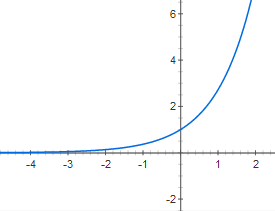
\includegraphics[width=0.5\columnwidth]{e_x}
\begin{itemize}[leftmargin=*]
  \item $y = \log_a x \Leftrightarrow x = a^y$
  \item $\log_a 1 = 0$
  \item $\log_a a^x = x$
  \item $a^{\log_a x} = x $
  \item $\log_a xy = \log_a x + \log_a y$
  \item $\log_a \frac{1}{x} = - \log_a x$
  \item $\log_a x^r = r \log_a x$
  \item $\log_a x = \frac{\log_b x}{\log_b a}$
  \item $\log_a x = \frac{\ln x}{\ln a}$
  \item $\log_a (x+y) = \log_a x + log_a (1 + \frac{y}{x})$
  \item $\log_a (x-y) = \log_a x + \log_a (1- \frac{y}{x})$
  \item $e^{a+bi} = e^a(\cos(b) + i \sin(b))$ (Euler Identität)
  \item $e^{b \ln(a)} = a^b$
  \item $ e^{-\ln(b)} = \frac{1}{b}$
\end{itemize}

\subsection{Komplexe Zahlen}
\begin{itemize}[leftmargin=*]
	\item $z \in \C: z = a + b\cdot i$
	\item $\bar{z} = a - b\cdot i$
	\item $|z|^2 = z \cdot \bar{z} = (a + b\cdot i) \cdot (a - b\cdot i) = a^2 + b^2$
	\item $i^2 = -1$
	\item $(a + bi) + (c + di) = (a + c) + (b + d)i$
	\item $(a + bi) \cdot (c + di) = (ac - bd) + (ad + bc)i$
	\item $\frac{a + bi}{c + di} = \frac{ac + bd}{c^2 + d^2} + \frac{bc - ad}{c^2 + d^2}\cdot i$
\end{itemize}

\subsection{Geometrische Körper}
\subsubsection{Ellipsoid}
Hat die Form eines Rugbyballs. In kartesischen Koordinaten definert durch
$\frac{x^2}{a^2} + \frac{y^2}{b^2} + \frac{z^2}{c^2} - 1 = 0$.

\subsection{Geometrie in 3D}
%evtl. nicht nötig. Aber in alten prüfungen oft gefragt.
\subsubsection*{Masse von speziellen Gebieten}
	\begin{multicols}{2}
	\renewcommand\arraystretch{1.4}
	\begin{tabular}{l|l}
		Zylinder   &   $ V = \pi r^2 h $ \\
		Pyramide   &   $ V = \frac{1}{3} G h $ \\
		Ellipsoid   &   $ V = \frac{4 \pi}{3} a b c $ \\
		Kegel   &   $ V = \frac{\pi}{3} r^2 h $ \\
		Kegelstumpf   &   $ V = \frac{\pi h}{3} (r_1^2+r_2^2 + r_1 r_2) $ 
	\end{tabular}
	
	\columnbreak
	\begin{tabular}{l|l}
		Torus   &   $ V = 2 \pi^2 R r^2 $ \\
		   &   $ S = 4 \pi^2 R r $ \\
		Kugel   &   $ V = \frac{4 \pi}{3} r^3 $ \\
		   &   $ S = 4 \pi r^2 $ 
	\end{tabular}
	\end{multicols}

 \subsubsection*{Rotationskörper}
 Rotation um die x Achse $V=\pi \int_a^b f(x)^2 dx.$\\
 Rotation um die y Achse $V=2\pi \int_a^b x \cdot f(x) dx.$



\subsection{Ausklammern}
\begin{itemize}[leftmargin=*]
	\item $x^n - y^n = (x-y) (x^{n-1} + x^{n-2}y + x^{n-3}y^2 + \ldots + xy^{n-2}
	+ y^{n-1})$
	\item $x^n - 1 = (x-1)(x^{n-1} + x^{n-2} + \ldots + x + 1)$
\end{itemize}

\subsection{Aus Serien}
\begin{itemize}[leftmargin=*]
	\item Ableitung von $x^x$ kann man berechnen, indem man $x = e^{\log(x)}$
	setzt. Also in diesem Fall $e^{\log(x^x)} = e^{x \log(x)}$ ableitet, was $e^{x
	\log(x)} (1 + \log(x))$ (Serie 10)
	\item Cauchy-Schwarz Ungleichung: $|x \cdot y| \leq \|x\| \cdot \|y\|, \; x,y \in \R^n$
	\item Euler Identität (komplexe Zahlen): $e^{ix} = \cos(x) + i \sin(x)$
\end{itemize}

\begin{landscape}\begin{multicols}{3}


\subsection{Funktionsgraphen}
\subsection*{\texorpdfstring{$\log(x)$}{log(x)}}
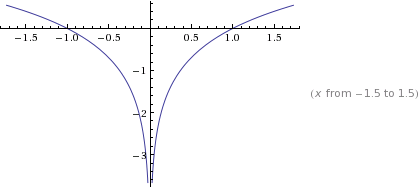
\includegraphics[scale=0.5]{log_x.png}

\subsection*{\texorpdfstring{$\frac{1}{x}$}{1/x}}
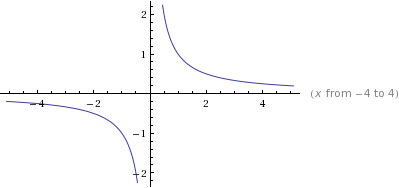
\includegraphics[scale=0.5]{1_over_x.png}

\subsection*{\texorpdfstring{$\sqrt{x}$}{x^(1/x)}}
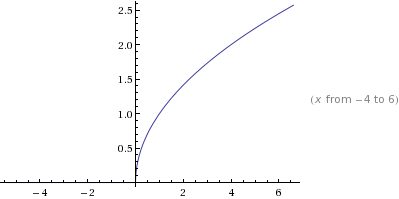
\includegraphics[scale=0.5]{sqrt_x.png}

\subsection*{Funktionsmanipulation}
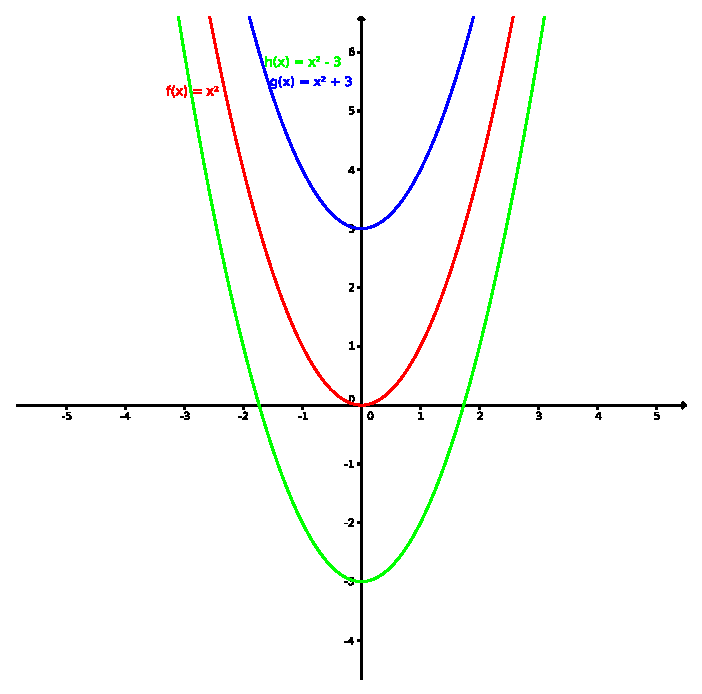
\includegraphics[width=\columnwidth]{manipulation_1.eps}
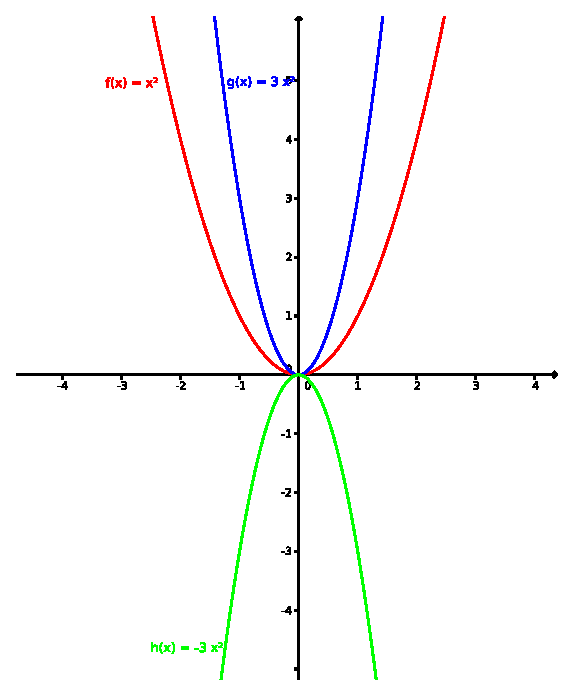
\includegraphics[width=\columnwidth]{manipulation_2.eps}
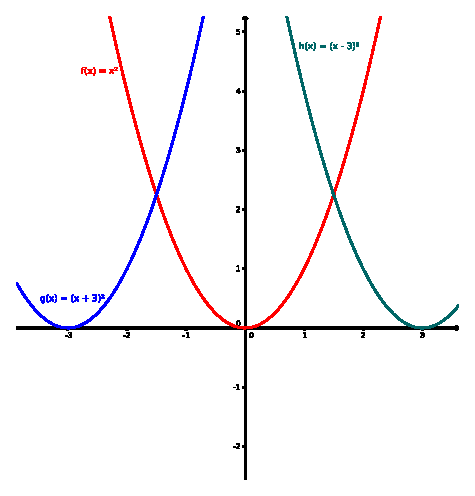
\includegraphics[width=\columnwidth]{manipulation_3.eps}

\subsection{Pascalsches Dreieck}
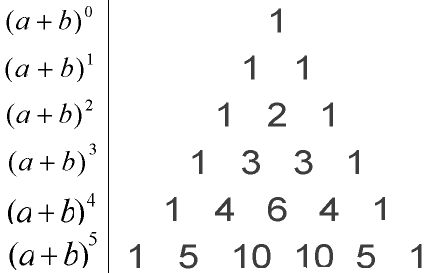
\includegraphics[width=\columnwidth]{pascal.png}

\end{multicols}\end{landscape}

%\onecolumn
\begin{landscape}
\section{Reihen Tabellen}

\begin{tabular}{|p{5cm}||p{5cm}|p{4cm}|p{4cm}|p{4cm}|p{4cm}|}
\hline & \multicolumn{4}{l}{schnelles Fallen} & langsames Fallen \\
\hline
 
wie schnell gehen die $a_n$ gegen 0 & exponentiell wie $q^n, |q| < 1$ &
polynominal wie $n^{-\alpha}, \alpha > 1$ & \multicolumn{2}{|c|}{höchstens wie
$1/n$} & gar nicht \\ \hline

Beispiele & \begin{align*} a_n = \frac{n^8}{2^n},\\ a_n =
(\sqrt[n]{n} - 1)^n,\\
a_n = \frac{1}{n!},\\ a_n = \left( \frac{-1}{4}\right)^n \end{align*} &
\begin{align*} a_n = \frac{1}{n^2}, \\ a_n = \frac{1}{n^{100}}, \\ a_n =
\frac{1}{(n + \ln n)^2}, \\ a_n = \frac{20}{n^2 - 33} \end{align*} &
\begin{align*} a_n = \frac{(-1)^n}{\ln n}, \\ a_n = \frac{(-1)^n}{n}
\end{align*} & \begin{align*} a_n = \frac{1}{\ln n}, \\ a_n = \frac{1}{n + \ln
n}, \\ a_n = \frac{1}{n} \end{align*} & \begin{align*} a_n = (-1)^n, \\ a_n =
\sin n, \\ a_n = n^2 \end{align*}\\ \hline

passende Konvergenzkriterien & Wurzel- und Quotientenkriterium & Integral- und
Verdichtungskriterium & Leibniz-Kriterium & & $a_n \not\to 0$ \\ \hline

Vergleichs-, Majoranten-, Minorantenkriterium & Vergleichen mit $q^n$ &
Vergleichen mit $n^{-\alpha}$ & kein Vergleich möglich & Vergleichen mit
$\frac{1}{n}$ & \\ \hline

Konvergenz-verhalten & \multicolumn{2}{c|}{absolute Konvergenz} & keine
absolute Konvergenz (einfach Konvergenz) & \multicolumn{2}{|c|}{Divergenz} \\
\hline

\end{tabular}

\begin{tabular}{|p{4cm}|p{15cm}|}\hline
\multicolumn{2}{|c|}{direkte Kriterien}\\ \hline

\textbf{Quotientenkriterium} & Gut für Reihen, die Fakultäten oder Glieder der
Form $a^n$ enthalten. Nicht auf Reihen anwendbar, in denen die Glieder nur wie
eine Potenz von $n$ fallen. \\ \hline

\textbf{Wurzelkriterium} & Gut in Reihen, deren Glieder $n$-te Potenzen sind,
zusammen mit der Stirlingformel oft auch bei Fakultäten anwendbar. \\ \hline

\textbf{Leibnizkriterium} & Nur für alternierende Reihen.\\ \hline

\textbf{Integralkriterium} & Anwendbar auf monotone Reihen.\\ \hline

\multicolumn{2}{|c|}{direkte Kriterien}\\ \hline

\textbf{Vergleichskriterium} & Ermöglicht es "`Störterme"' wegzulassen und so
einfachere Reihen zu untersuchen \\ \hline

\textbf{Verdichtungskriterium} & Bei monotonen Reihen anwendbar. Für Reihen mit
langsam fallenden Gliedern \\ \hline

\textbf{Majoranten- und Minorantenkriterium} & Ähnlich wie Vergleichskriterium.
Wird mit einer Reihe verglichen, deren Glieder stets kleiner oder grösser sind.
\\ \hline
\end{tabular}

\end{landscape}
\twocolumn

\part{Generelles}

\section{Trigonometrische Definitionen \& Sätze}
\subsection{Definitionen}

$sin(x) := \sum_{n=0}^{\infty} (-1)^n \frac{x^{2n+1}}{(2n+1)!} = \frac{x}{1!} - \frac{x^3}{3!} + \frac{x^5}{5!} \mp ...$

$cos(x) := \sum_{n=0}^{\infty} (-1)^n \frac{x^{2n}}{(2n)!} = \frac{x^0}{0!} - \frac{x^2}{2!} + \frac{x^4}{4!} \mp ...$

$exp(x) := \sum_{n=0}^{\infty} \frac{x^{n}}{n!} = \lim\limits_{n \rightarrow \infty}{(1 + \frac{x^{n}}{n})^n}$

$arctan(x) := \sum_{n=0}^{\infty} (-1)^n \frac{x^{2n+1}}{2n+1} = \frac{x}{1} - \frac{x^3}{3} + \frac{x^5}{5} \mp ...$

Hinweis: Für einfache Approximation genügt es die ersten paar Glieder der $arctan(x)-Reihe$ zu berechnen. \newline 
Falls: $x \notin [0,1]$, gibt es eine Vereinfachung:
$ arctan(x) = \frac{sgn(x) * \pi}{2} - arctan(\frac{1}{x}) $

\subsubsection{Definition Taylorreihe} Eine Funktion $f(x)$ wird an einer Stelle $x_0$ angenähert durch $Tf(x;x_0) = \sum_{n=0}^{\infty} \frac{f^{(n)}(x_0)}{n!}(x - x_0)^n = f(x_0)$ \\

\subsubsection{Definitionen csc(x), sec(x), cot(x)}
$csc(x) := \frac{1}{sin(x)}$ \hfil $sec(x) := \frac{1}{cos(x)}$ \hfil $cot(x) := \frac{1}{tan(x)} = \frac{cos(x)}{sin(x)}$





\subsection{Periodizit"aten}

\begin{minipage}{0.49\linewidth}

\begin{itemize}
	\item \(1\cdot e^{2\pi i k} = 1\) f"ur alle \(k \in \mathbb{Z}\)
	\item	\(e^{\frac{\pi}{2} i k} = i\)
	\item \(e^{-\frac{\pi}{2} i k} = -i\)
	\item \(e^{-2 \pi i k} = 1\)
	\item \(e^{\pi i k} = (-1)^k\)
	\item \(e^{-\pi i k} = (-1)^k\)
\end{itemize}	

\end{minipage}
\hfill
\begin{minipage}{0.49\linewidth}
\begin{itemize}	
	\item $ \sin(z+2 \pi) = \sin(z) $
	\item $ \cos(z+2 \pi) = \cos(z) $
	\item $\sinh(z + 2 \pi i) = \sinh(z)$
	\item $\cosh(z + 2 \pi i) = \cosh(z)$
	\item $ \sin(z- \pi) = -\sin(z) $
	\item $ \cos(z- \frac{\pi}{2}) = \sin(z) $
\end{itemize}
\end{minipage}
\subsection{Winkel}
\renewcommand{\arraystretch}{1.5}
\begin{tabular}{|c|c|c|c|c|c|c|c|c|}
	\hline
	\(\varphi \) &$0$ & \(\frac{\pi}{6}\) & \(\frac{\pi}{4}\) & \(\frac{\pi}{3}\) &  \(\frac{\pi}{2}\) &  \(\frac{2\pi}{3}\) &  \(\frac{3\pi}{4}\) & \(\frac{5\pi}{6}\) \\
	\hline
	Grad & $0^\circ$ & $30^\circ$ & $45^\circ$ & $60^\circ$ & $90^\circ$ & $ 120^\circ$ & $135^\circ$ & $150^\circ$\\
	\hline
	\(\sin(\varphi)\) & $0$ & \(\frac{1}{2}\) & \(\frac{\sqrt{2}}{2}\) & \(\frac{\sqrt{3}}{2}\) & $1$ &  \(\frac{\sqrt{3}}{2}\) &  \(\frac{1}{\sqrt{2}}\) &  \(\frac{1}{2}\)   \\
	\hline
	\(\cos(\varphi)\) &$1$ & \(\frac{\sqrt{3}}{2}\) & \(\frac{\sqrt{2}}{2}\) & \(\frac{1}{2}\) & $0$ & $-\dfrac{1}{2}$ & \(-\frac{1}{\sqrt{2}}\) &  \(-\frac{\sqrt{3}}{2}\)  \\
	\hline
	\(\tan(\varphi)\) &$ 0$ & \(\frac{1}{\sqrt{3}}\) &  $1$ & $\sqrt{3}$ & $\pm \infty$ &$-\sqrt{3}$ & $-1$ &  \(-\frac{1}{\sqrt{3}}\)\\ 
	\hline
\end{tabular}\\

\begin{tabular}{|c|c|c|c|c|c|c|c|}
	\hline
	\(\varphi \) &$\pi$ & \(\frac{7\pi}{6}\) & \(\frac{5\pi}{4}\) & \(\frac{4\pi}{3}\) &  \(\frac{3\pi}{2}\) &  \(\frac{5\pi}{3}\) &  \(\frac{7\pi}{4}\)  \\
	\hline
	Grad & $180^\circ$ & $210^\circ$ & $225^\circ$ & $240^\circ$ & $270^\circ$ & $ 300^\circ$ & $315^\circ$\\
	\hline
	\(\sin(\varphi)\) & $0$ & \(-\frac{1}{2}\) & \(-\frac{\sqrt{2}}{2}\) & \(-\frac{\sqrt{3}}{2}\) & $-1$ &  \(-\frac{\sqrt{3}}{2}\) &  \(-\frac{1}{\sqrt{2}}\)  \\
	\hline
	\(\cos(\varphi)\) &$-1$ & \(-\frac{\sqrt{3}}{2}\) & \(-\frac{\sqrt{2}}{2}\) & \(-\frac{1}{2}\) & $0$ & $\dfrac{1}{2}$ & \(\frac{1}{\sqrt{2}}\)  \\
	\hline
	\(\tan(\varphi)\) &$ 0$ & \(\frac{1}{\sqrt{3}}\) &  $1$ & $\sqrt{3}$ & $\pm \infty$ &$-\sqrt{3}$ & $-1$ \\ 
	\hline
\end{tabular}\\
\renewcommand{\arraystretch}{1.0}

\newpage
\subsection{Sinusssatz}
\begin{figure}[h!]
\centering
    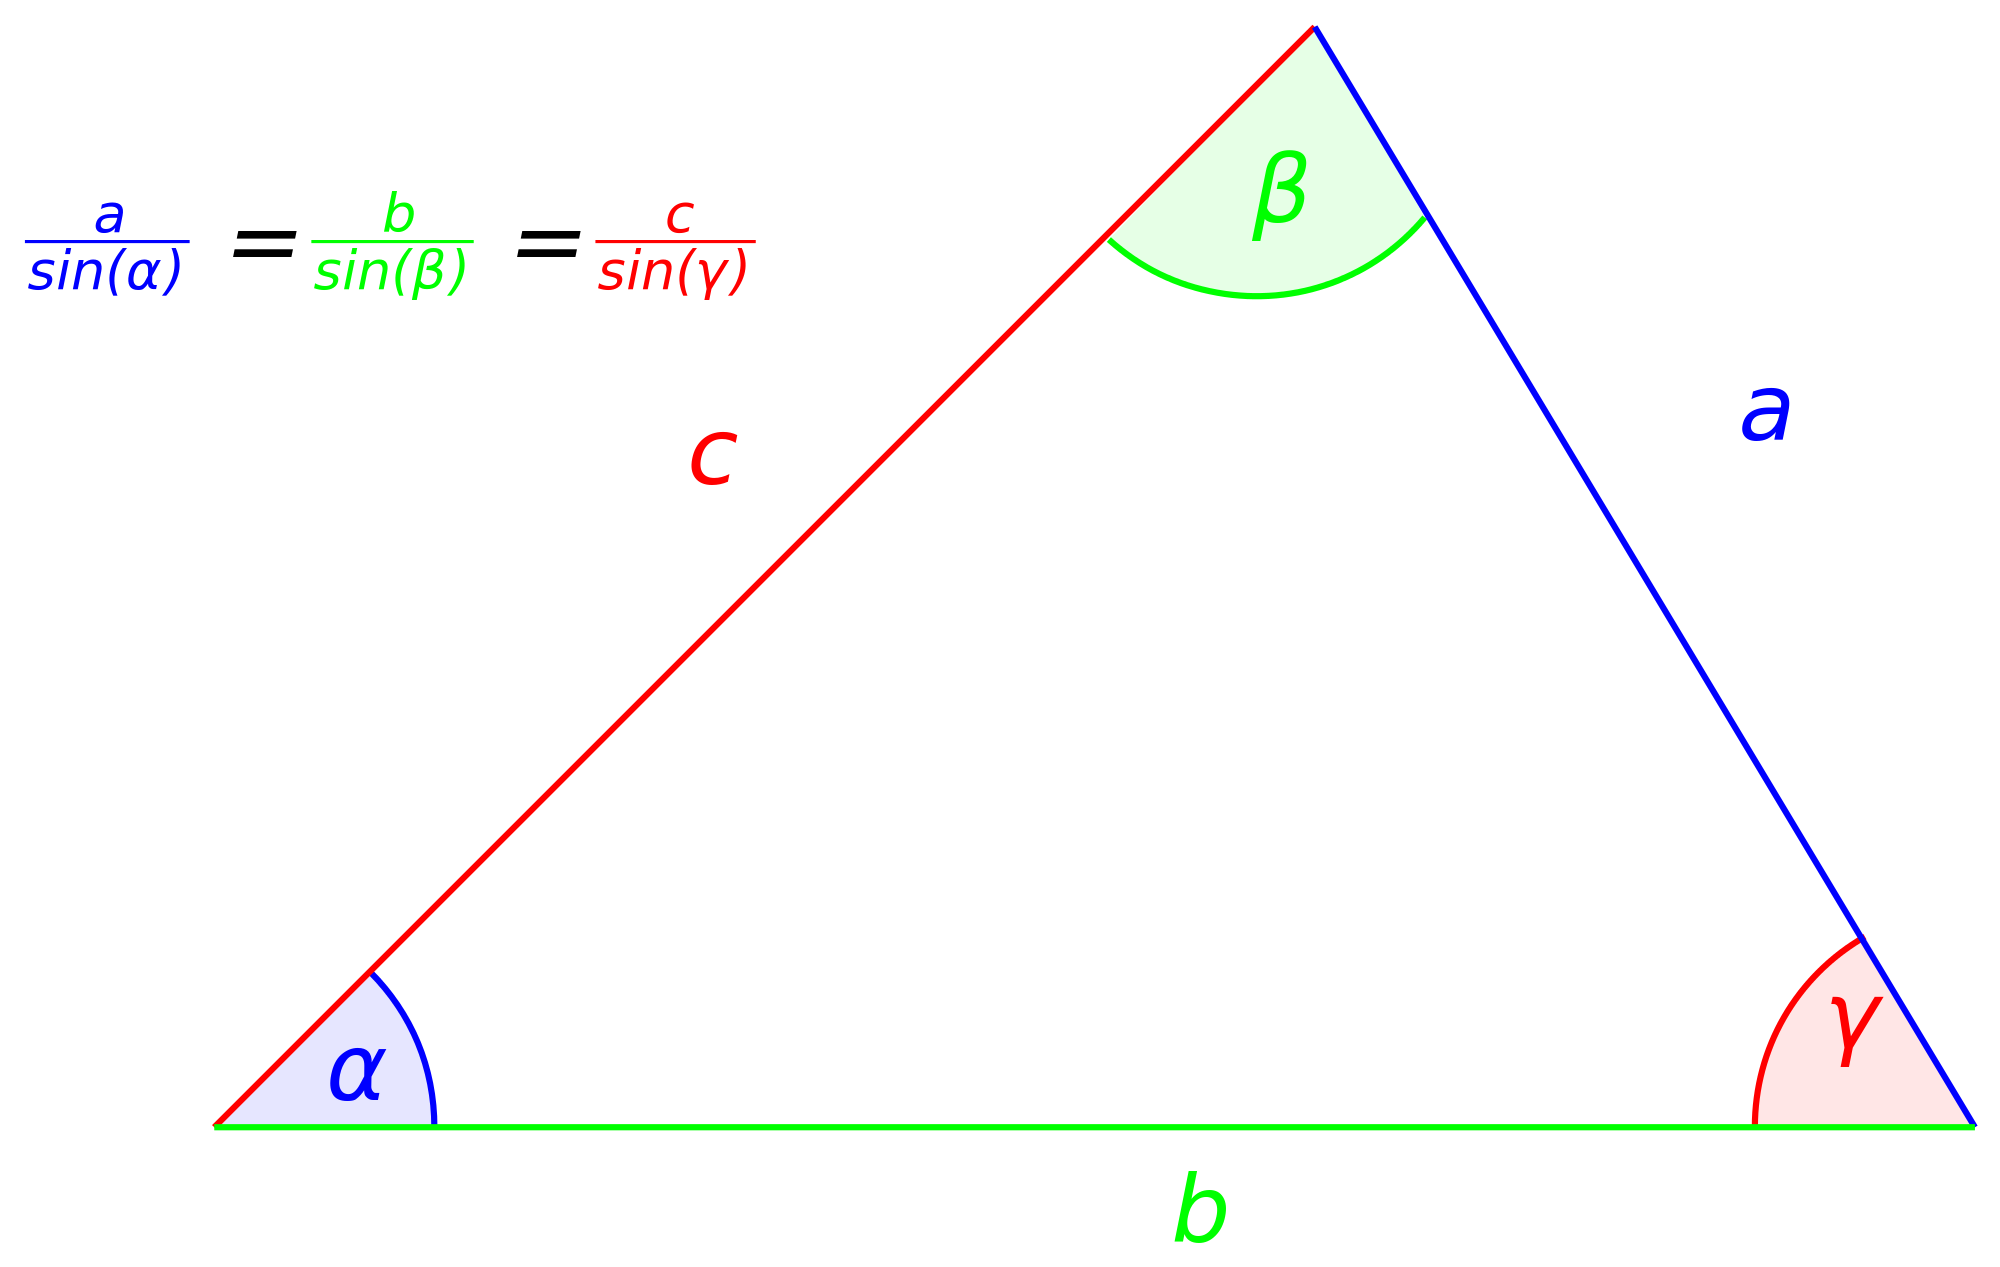
\includegraphics[width=0.5\textwidth]{images/sinussatz.png}
    \caption{Quelle: https://de.wikipedia.org/}
    
\end{figure}
\subsection{Cosinusssatz}
$a^2 + b^2 -2ab*cos(\gamma)= c^2$


\subsection{Standardintegrale}
\begin{minipage}{0.49\linewidth}
$\frac{d}{dx} arcsin(x) = \frac{1}{\sqrt{1-x^2}}$ \\
$\frac{d}{dx} arccos(x) = \frac{-1}{\sqrt{1-x^2}}$ \\
$\frac{d}{dx} arctan(x) =\frac {1}{x^2+1}$ \\
\end{minipage}
\begin{minipage}{0.49\linewidth}
$\frac{d}{dx} arsinh(x) =\frac{1}{\sqrt{x^2+1}}$ \\
$\frac{d}{dx} arcosh(x) =\frac{1}{\sqrt{x^2-1}}, $wenn $ x>1$ \\
$\frac{d}{dx} artanh(x) =\frac{1}{1-x^2}, $wenn $ |x|<1$ \\
\end{minipage}

\subsection{Euler Formel}
$exp(i \phi) = cos(\phi) + isin(\phi)$
\\
$exp(-i \phi) = cos(-\phi) + isin(-\phi) \Longleftrightarrow $ 
$exp(-i \phi) = cos(\phi) - isin(\phi)$ 

Daraus kann nun sin, sinh, cos und cosh in Termen von exp(x) ausgedrückt werden.

$\frac{exp(i \phi) + exp(-i \phi)}{2}  = cos(\phi)$\\
$\frac{exp(i \phi) - exp(-i \phi)}{2i}  = sin(\phi)$

Ignoriere alle i, dann folgt...

$\frac{exp(\phi) + exp(-\phi)}{2}  = cosh(\phi)$\\
$\frac{exp(\phi) - exp(-\phi)}{2}  = sinh(\phi)$




\subsection{Ableitungen, Integrale}
\subsection{Ableitungen}
$\frac{d}{dx}sin(x) = cos(x)$

$\frac{d}{dx}cos(x) = -sin(x)$

$\frac{d}{dx}tan(x) = \frac{d}{dx} \frac{sin(x)}{cos(x)} = \frac{cos(x)cos(x)- sin(x)sin(x)}{cos^2(x)} = 1 - \frac{sin^2(x)}{cos^2(x)} = 1 - tan^2(x) = \frac{1}{cos^2(x)}$

$\frac{d}{dx} \frac{1}{sin(x)} = \frac{0*sin(x) - 1*cos(x)}{sin^2(x)} = \frac{-cos(x)}{sin^2(x)}$ 

$\frac{d}{dx} \frac{1}{cos(x)} = \frac{0*cos(x) - 1*(-sin(x))}{cos^2(x)} = \frac{sin(x)}{cos^2(x)}$

$\frac{d}{dx}sin^2(x) = sin(x)*cos(x)+ cos(x)*sin(x) = 2*sin(x)*cos(x)$

$\frac{d}{dx}cos^2(x) = cos(x)*(-sin)(x)+ (-sin(x))*cos(x) = -2*sin(x)*cos(x)$ 
\newpage
\subsection{Rechenregeln}
\subsection{Additionstheoreme}
$sin^2(x)+cos^2(x) = 1$

$sin(x \pm y) = sin(x)cos(y) \pm cos(x)sin(y)$    \ \ $(\# umgekehrteAbleitungsregel)$

$cos(x \pm y) = cos(x)cos(y) \mp \sinx \siny$

$tan(x \pm y) = \frac{\tanx \pm \tany}{ 1 \mp \tanx \; \tany } = \frac{ sin(x \pm y) }{cos(x \pm y) }$

\subsection{Doppelwinkel}
$sin(2x)= 2\sinx \cosx = \frac{2 \tanx}{ 1 + tan^2(x) }$

$cos(2x)= cos^2(x) - sin^2(x) = 1 - 2sin^2(x) = 2cos^2(x) - 1 = \frac{ 1 - tan^2(x) }{ 1 + tan^2(x) }$

$tan(2x)= \frac{ 2 \tanx }{ 1 - tan^2(x) } = \frac{2}{ cot(x) - \tanx }$

$cot(2x)= \frac{ cot^2(x) - 1}{2cot(x)} = \frac{cot(x) - \tanx}{2}$ \\

Beweis mit Additionstheorem



\subsection{Produkt-zu-Summen-Formel}
$\sinx*sin(y) = \frac{1}{2}(cos(x-y)-cos(x+y))$

$\cosx*cos(y) = \frac{1}{2}(cos(x-y)+cos(x+y))$

$sin(x)*cos(y) = \frac{1}{2}(sin(x-y)+sin(x+y))$ \\



\subsection{Hyperbolische Funktionen}
$sinh(z) := \frac{e^z - e^{-z}}{2} = z + \frac{z^3}{3!} + \frac{z^5}{5!} + \frac{z^7}{7!} + \dots = \sum_{n=0}^\infty \frac{z^{2n+1}}{(2n+1)!}$

$cosh(z) := \frac{e^z + e^{-z}}{2}= 1 + \frac{z^2}{2!} + \frac{z^4}{4!} + \frac{z^6}{6!} + \dots = \sum_{n=0}^\infty \frac{z^{2n}}{(2n)!}$

$sin(z)= Im(e^{iz})=\dfrac{1}{2i} (e^{iz}-e^{-iz})$ \\

$cos(z)=\text{Re}(e^{iz})=\dfrac{1}{2}(e^{iz}+e^{-iz})$ \\

$sinh(\pm iz) = \pm i \cdot \sin(z)$\\
$cosh(\pm iz) = cos(z)$\\
$sin(iz)= i\cdot sinh(z)$\\
$cos(iz)=cosh(z)$\\

$ \sin(-z) = - \sin(z) $\\
$ \tan-(z) = -\tan(z) $\\
$ \cos(-z) = \cos(z) $ \\
$ \arctan(-z) = -\arctan(z) $

$\sin(z) = \sin(x)\cosh(y) + i\cos(x)\sinh(y)$\\
$\cos(z) = \cos(x)\cosh(y) - i\sin(x)\sinh(y)$\\
$e^z = e^x \cos(y) + i e^x \sin(y)$\\
$\sinh(z) = \cos(y)\sinh(x) + i\sin(y)\cosh(x)$\\
$\cosh(z) = \cos(y)\cosh(x) + i\sin(y)\sinh(x)$	

\begin{itemize}[leftmargin=*]
	\item $\int \sinh(ax + b) \,dx = \frac{\cosh(ax + b)}{a}$; $\int \sinh(x) \,dx
	= \cosh(x)$
	\item $\int \cosh(ax + b) \,dx = \frac{\sinh(ax + b)}{a}$; $\int \cosh(x) \,dx
	= \sinh(x)$
	\item $\int \tan(ax + b) \,dx = \frac{\log(\cosh(ax+b))}{a}$; $\int \tan(x)
	\,dx = \log(\cosh(x))$
\end{itemize}


\subsection{Additionstheoreme}
$sinh(z_1 \pm z_2) = sinh(z_1) \cdot cosh(z_2) \pm sinh(z_2) \cdot cosh(z_1)$

$cosh(z_1 \pm z_2) = cosh(z_1) \cdot cosh(z_2) \pm sinh(z_1) \cdot sinh(z_2)$

$tanh(z_1 \pm z_2) = \frac{tanh(z_1) \pm tanh(z_2)}{1 \pm tanh(z_1) \cdot tanh(z_2)}$


\subsubsection{Zusammenhänge}
$cosh^2(z) - sinh^2(z) = 1$ \hfill $cosh(z) + sinh(z) = e^z$ \hfill $cosh(z) - sinh(z) = e^{-z}$

\subsection{Ableitungen}
$\frac{d}{dz}sinh(z) = cosh(z)$ \hfill $\frac{d}{dz}cosh(z) = sinh(z)$ \hfill $\frac{d}{dz}tanh(z) = 1 -tanh^2(z) = \frac{1}{cosh^2(x)}$

\section{Plots Trigonometrischer Funktionen}
%Alle Plots in diesem Kapitel von www.wikipedia.org!

\begin{figure}[!htb]
	\centering
	\begin{minipage}{.5\textwidth}
		\centering
		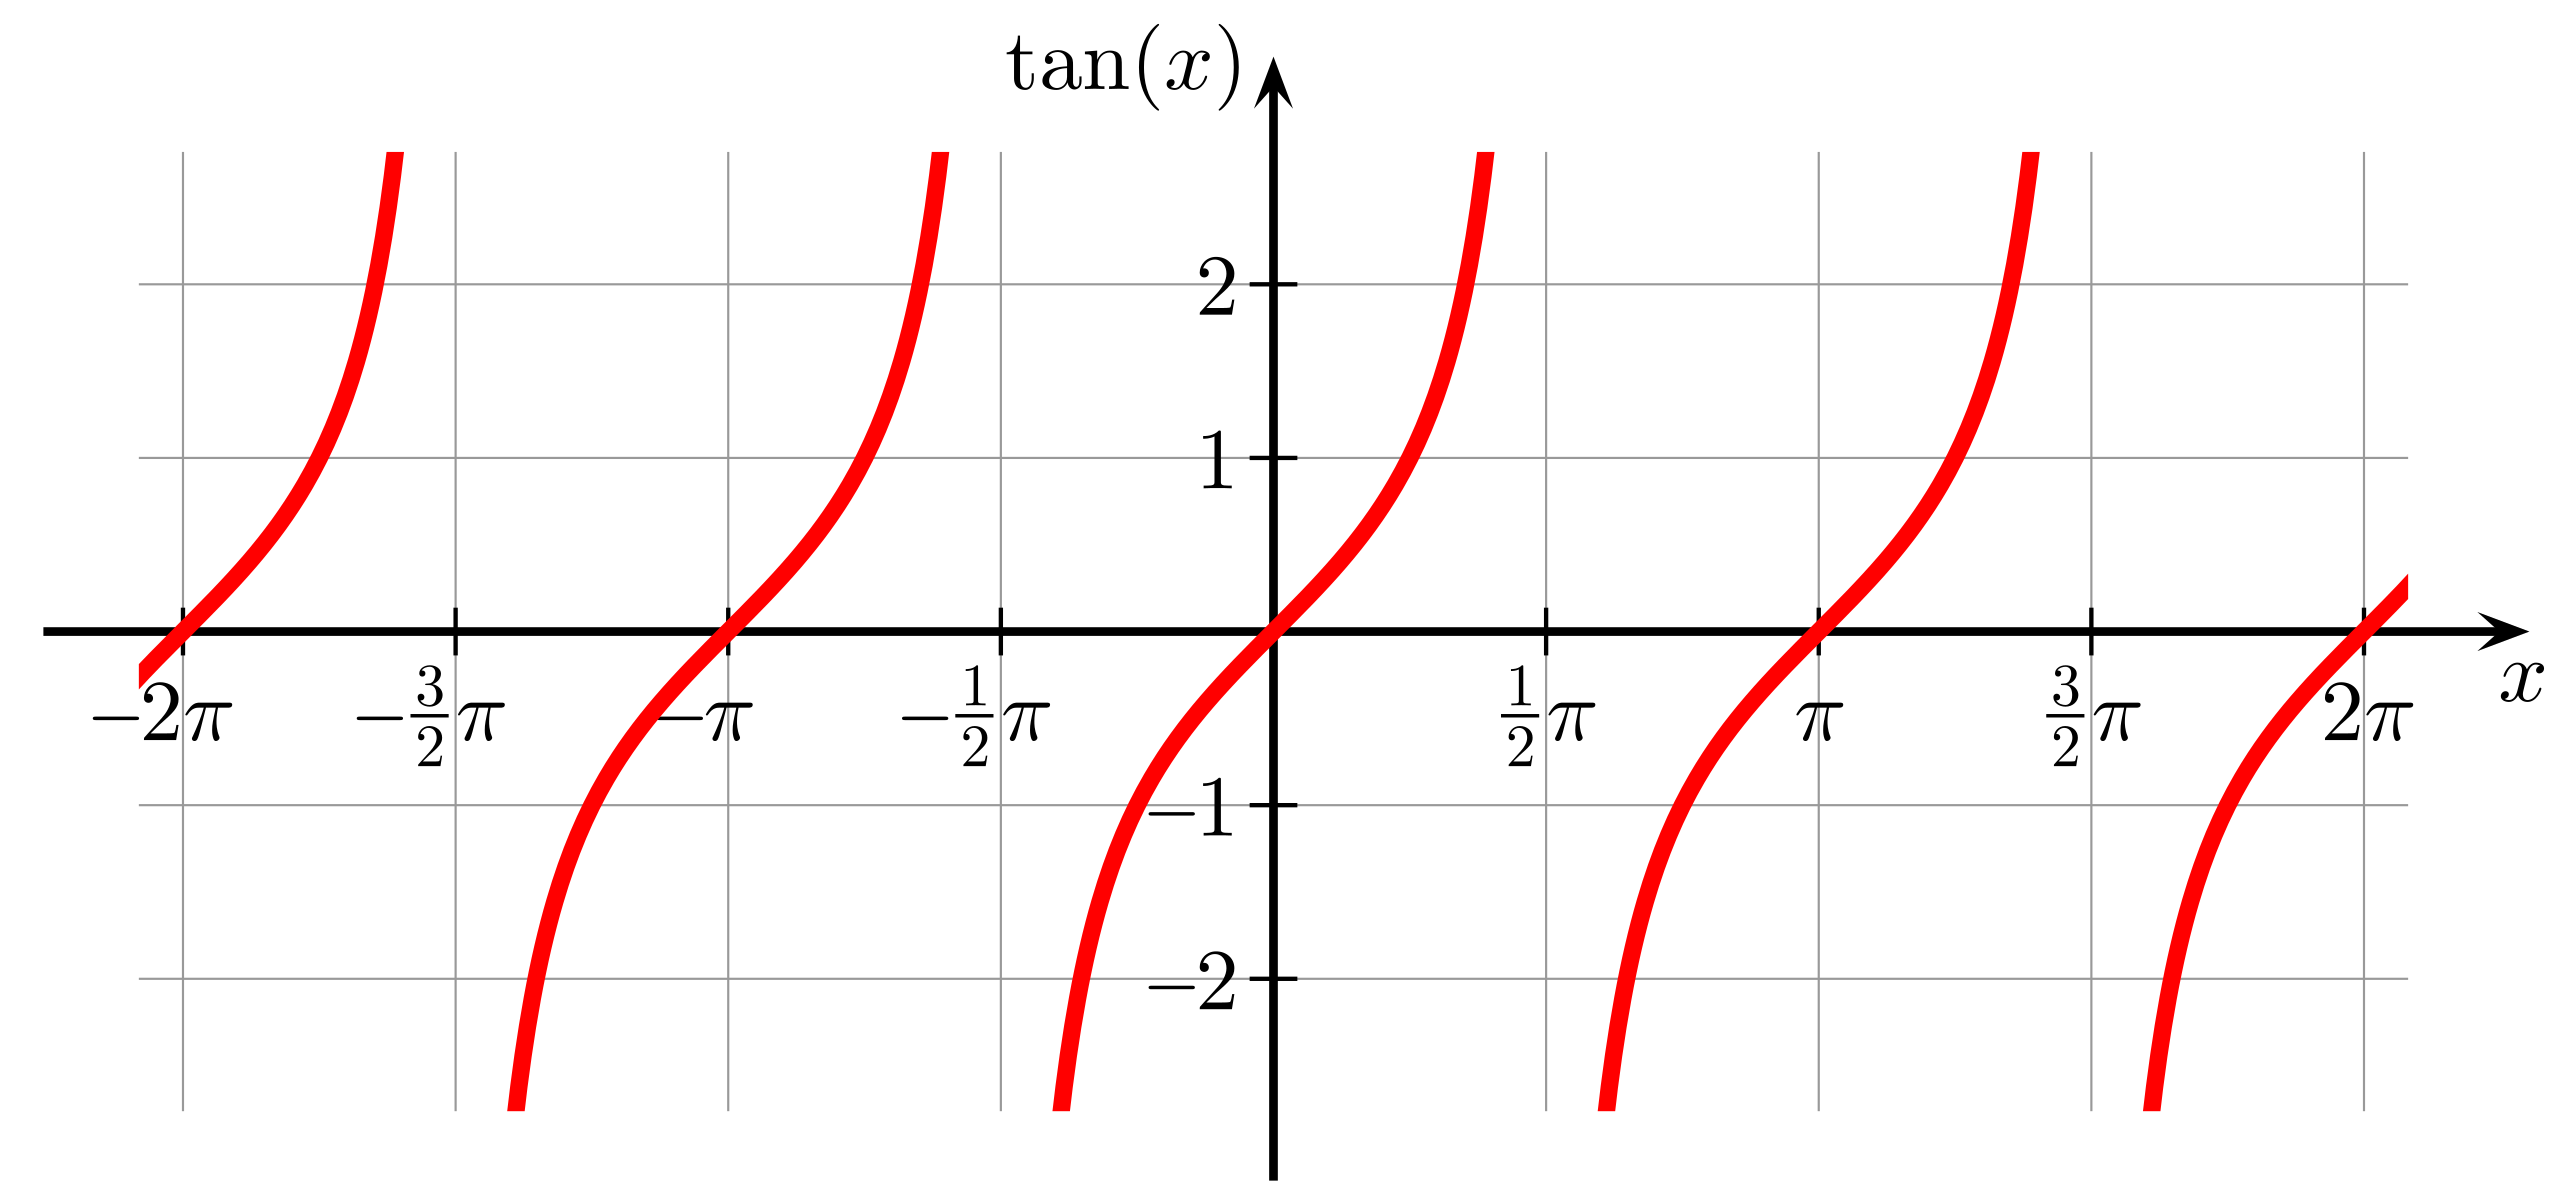
\includegraphics[width=1\linewidth]{images/tan.png}
	\end{minipage}%
	\begin{minipage}{0.5\textwidth}
		\centering
		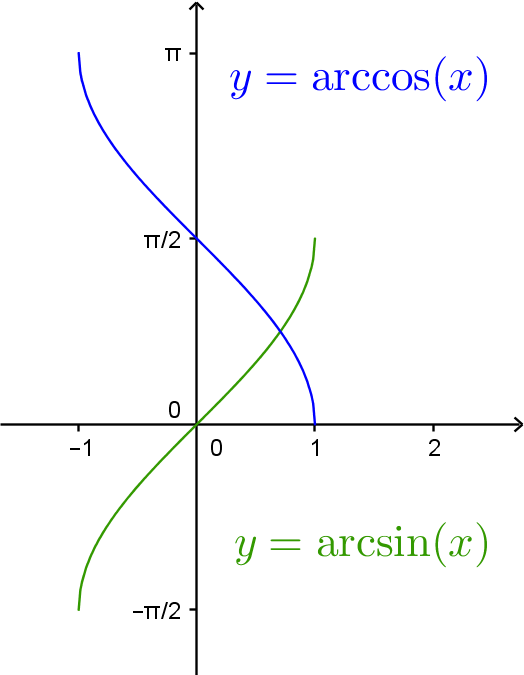
\includegraphics{images/asinacos.png}
	\end{minipage}
\end{figure}


\begin{figure}[H] 
	\centering
	{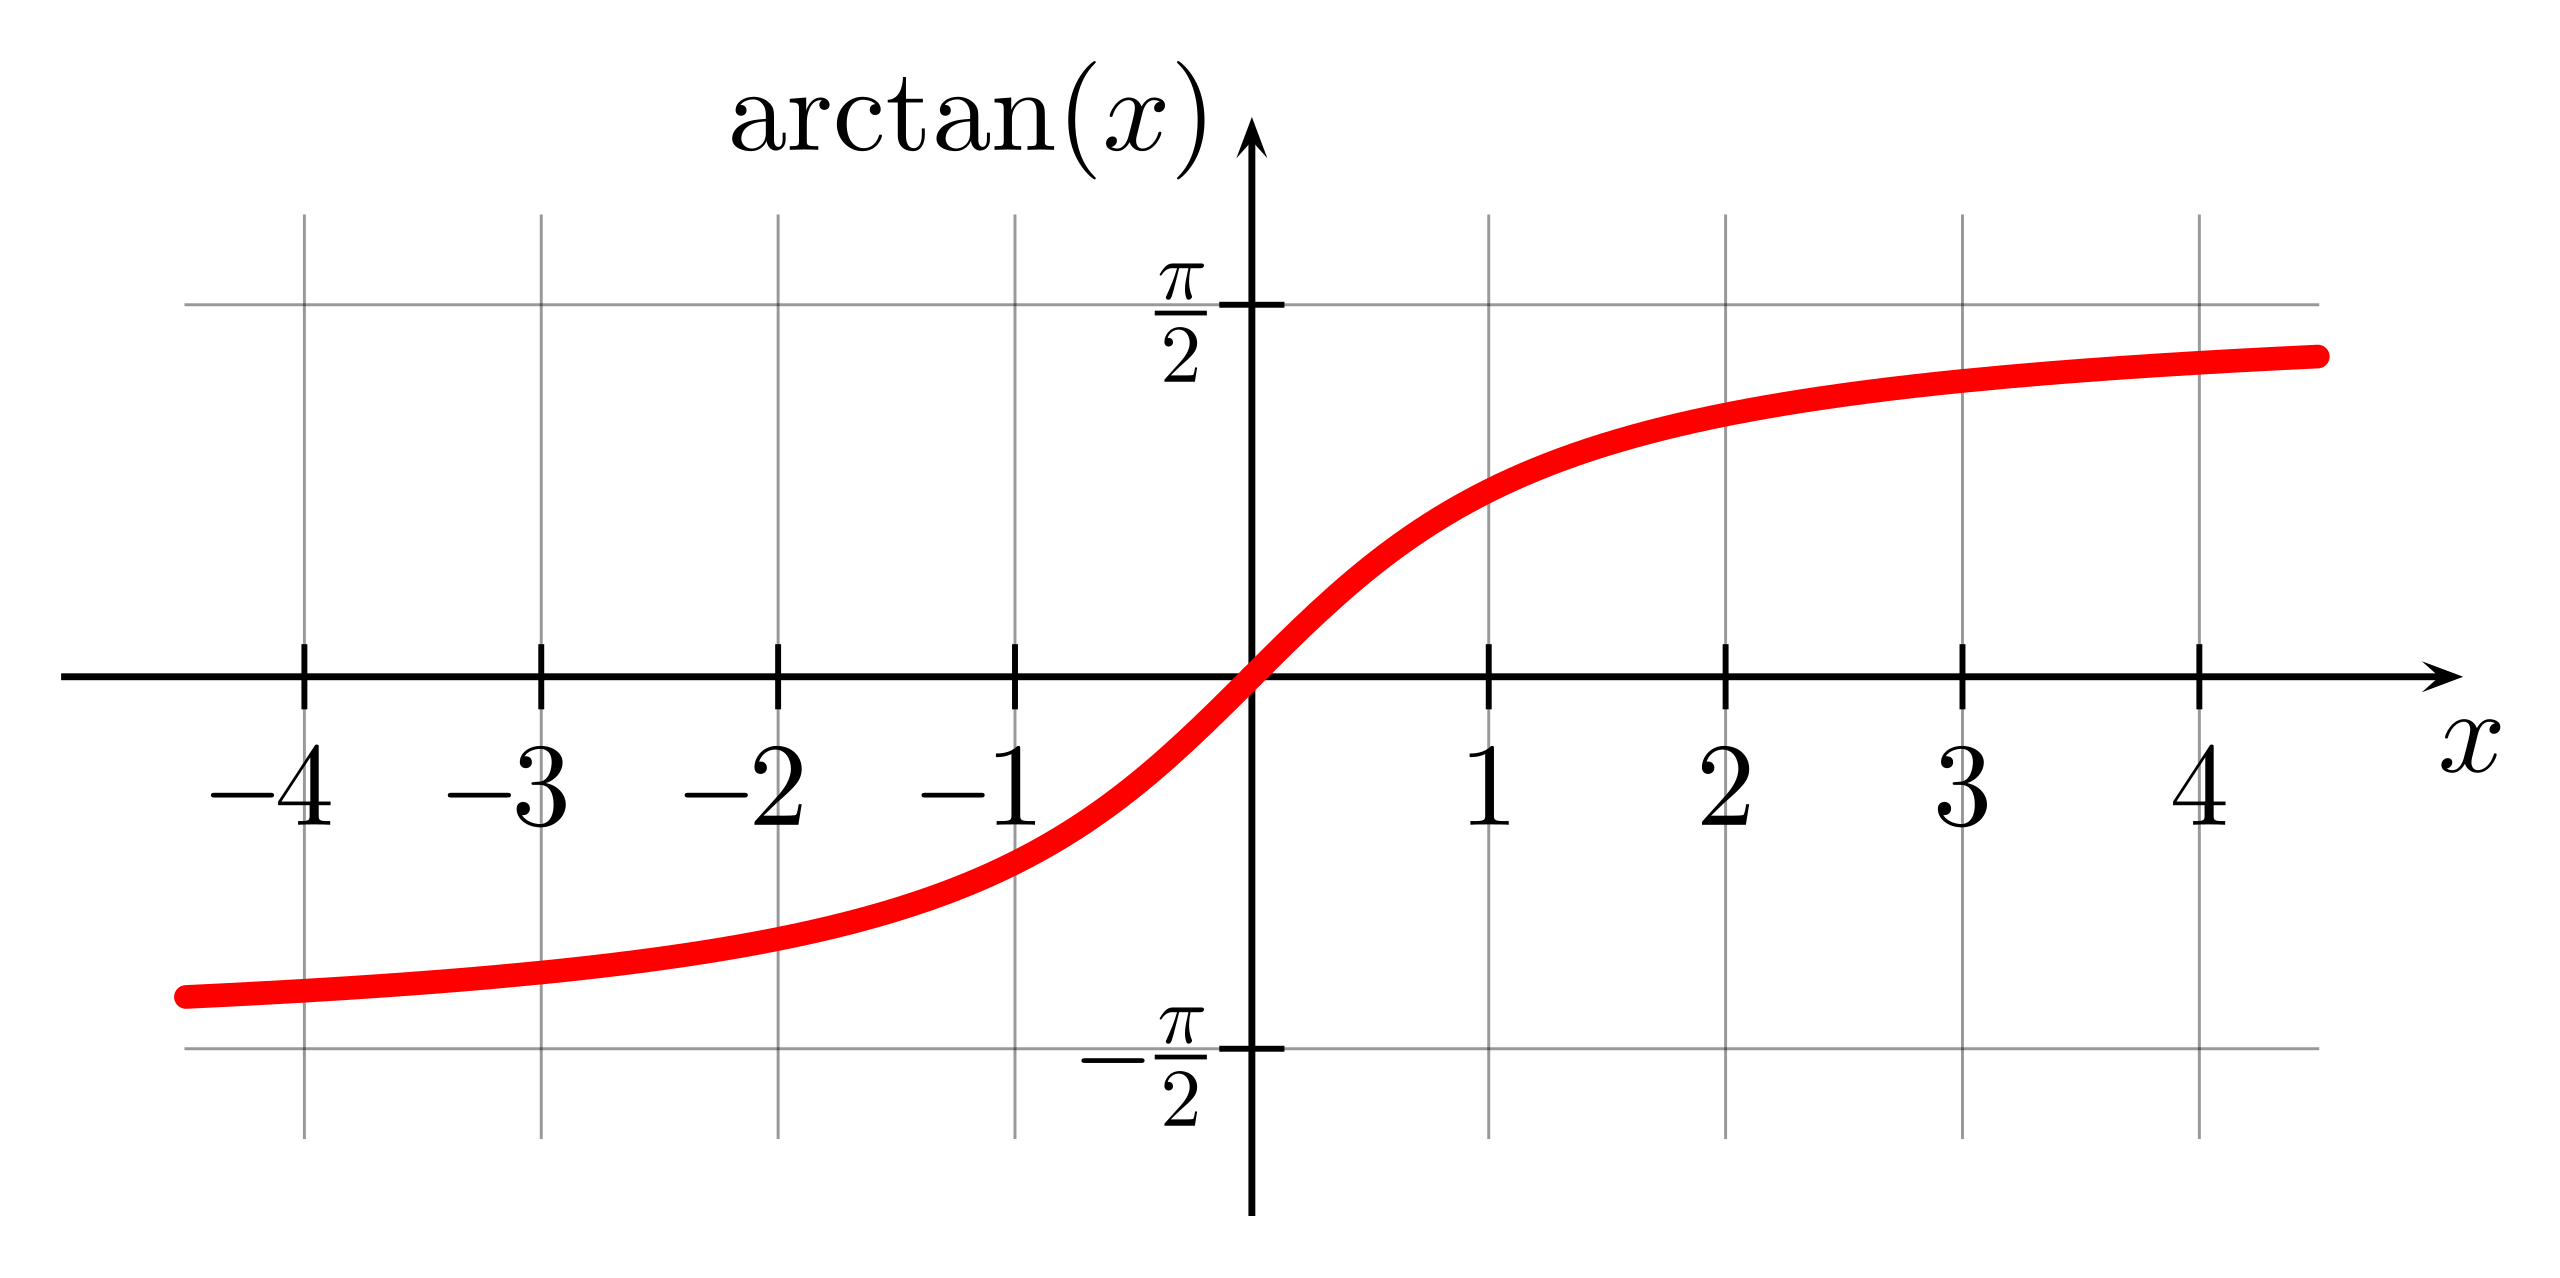
\includegraphics[width=0.55\textwidth]{images/arctan.png}}
\end{figure}



\begin{figure}[!htb]
	\centering
	\begin{minipage}{.5\textwidth}
		\centering
		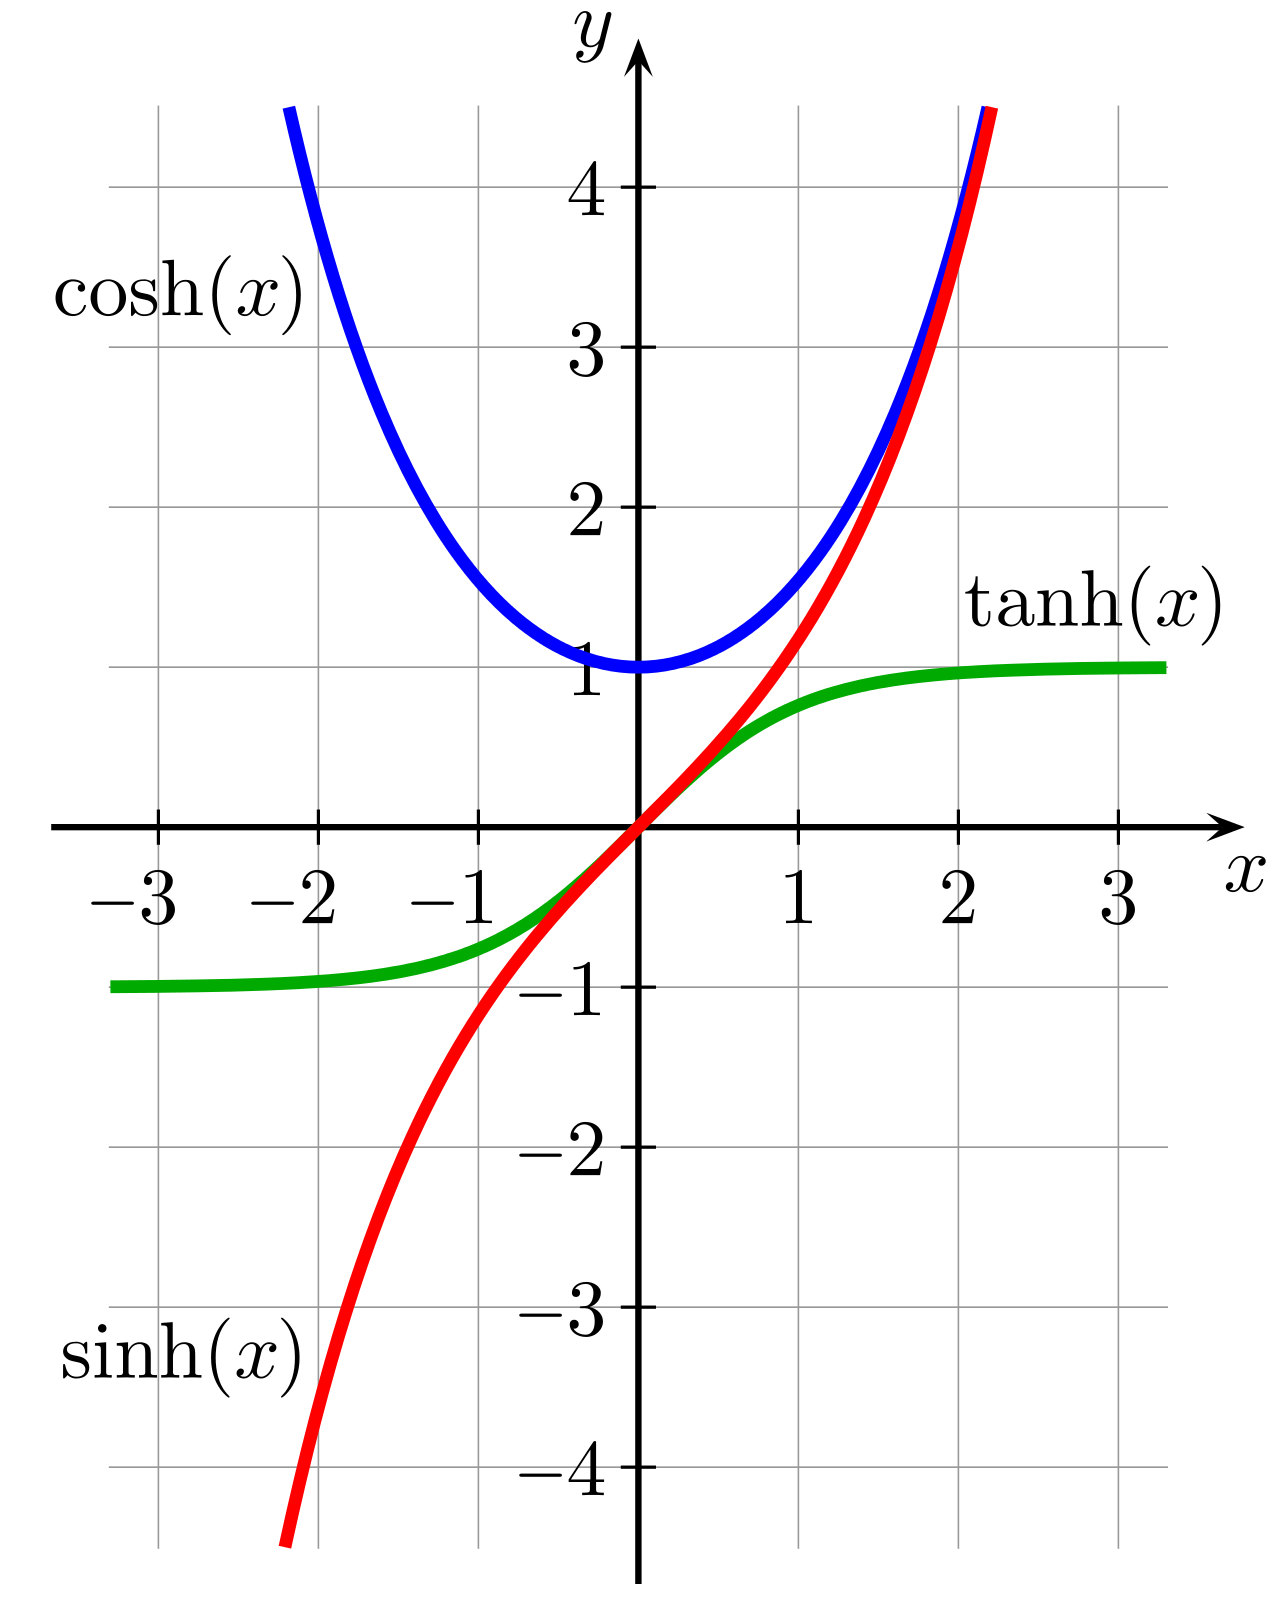
\includegraphics[width=1\linewidth]{images/sinhcoshtanh.png}
	\end{minipage}%
	\begin{minipage}{.5\textwidth}
		\centering
		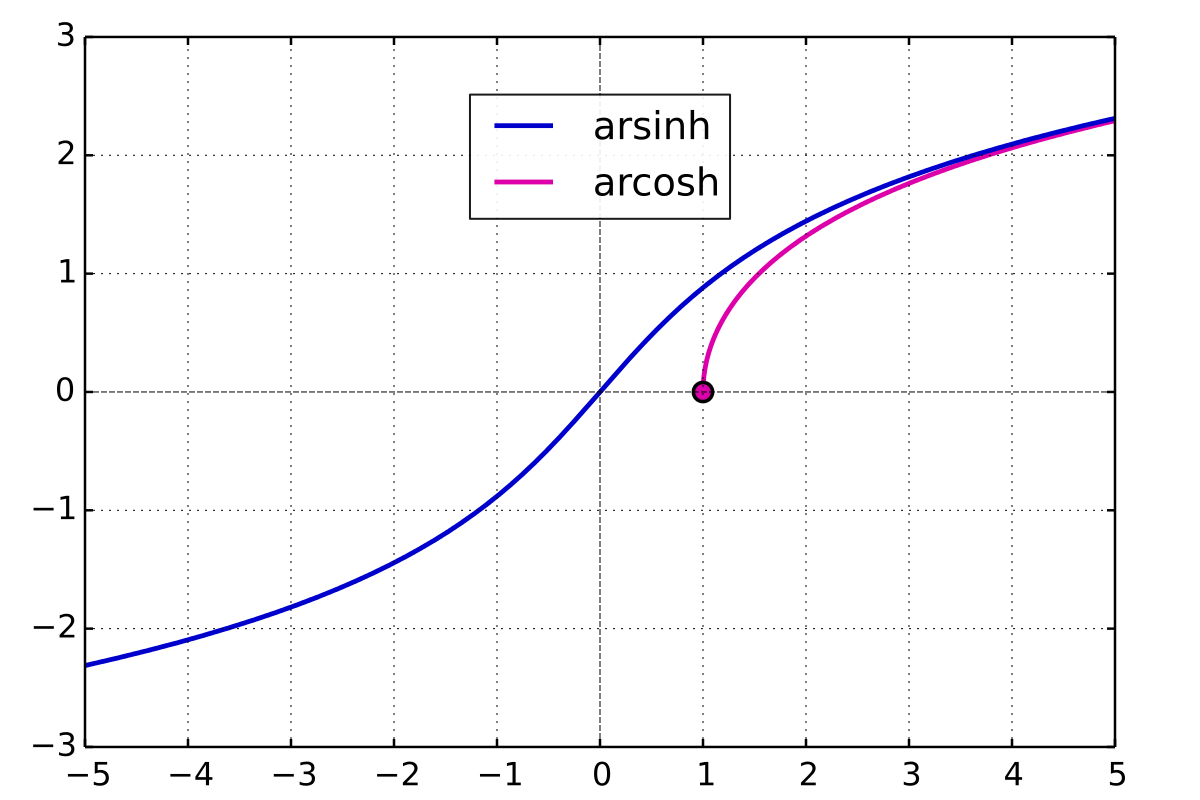
\includegraphics[width=1\linewidth]{images/arsinharcosh.png}
	\end{minipage}
\end{figure}


\section{Vollständige Induktion}\index{Induktion}
Grundlägende Struktur um die Aussage $A(n)$ zu beweisen:
\begin{enumerate}
	\item \textbf{Induktionsanfang/Verankerung:} Die Aussage wird für $n = A$ bewiesen.
	$A$ ist dabei meistens der erste Wert für die gegebene Eingabemenge.
	Der Beweis wird meist durch direktes ausrechnen gemacht.
	\item \textbf{Annahme/Induktionsvoraussetzung:} Hier schreibt man,
	dass man davon ausgeht die Aussage sei gültig (damit man sie im nächsten Schritt)
	einsetzen kann. Man kopiert also im Grunde, was man zu beweisen hat mit einigen Zierwörter.
	\item \textbf{Induktionsschritt:} Für jedes $n \geq A$ wird unter Benutzung der Aussage $A(n)$
	die Aussage $A(n+1)$ bewiesen. Dazu wird die Induktionsannahme verwendet.
\end{enumerate}

\subsection{Beispiel}
		Es ist zu beweisen, dass für jedes $n \in \N$ folgendes gilt: $1 + 2 + 3 + \ldots + n = \frac{n(n + 1)}{2}$		
		
		Lemma: $\forall \in \N. 1 + 2 + 3 + \ldots + n = \frac{n(n + 1)}{2}$ \\
		
	Beweis: \\
		  Sei $P(n) \equiv 1 + 2 + 3 + \ldots + n = \frac{n(n + 1)}{2}$. \\
		  Wir zeigen $\forall \in \N. P(n)$ mit vollständiger Induktion.\\
		
		Induktionsanfang: Zeige $P(0)$. \\
		 $$0 =  \frac{0(0 + 1)}{2}$$
		
		  Induktionsschritt: \\
		    Sei $n \in N$ beliebig und nehmen wir $P(n)$ an (Induktionsvoraussetzung).  \\
		    Zeige $P(n+1)$ (Induktionsbehauptung).\\
		  \begin{align}
		      1 + 2 + 3 + \ldots + n + (n + 1) =\\
		      = \frac{n(n + 1)}{2} + (n+1)       & \text{ — P(n) Induktionsvor. }\\
		      = \frac{n(n + 1)}{2} + \frac{2(n + 1)}{2}  & \text{—arith}\\
		      = \frac{(n+1)*((n+1)+1)}{2}        & \text{—arith}
		\end{align}
		qed.
\section{Mengen}

\subsection{Definitionen}

\begin{description}[labelindent=16pt,style=multiline,leftmargin=6cm, noitemsep]
	\item[Obere/Untere Schranke:] $\exists b \in \mathbb{R}\ \forall a\in A:\ a \leq b$, $\exists c \in \mathbb{R}\ \forall a\in A:\ a \geq c$
	\item[Supremum:] kleinste obere Schranke $\sup A$
	\item[Infimum:] gr{\"o}sste untere Schranke $\inf A$
	\item[Maximum/Minimum:] $\sup A \in A$, $\inf A \in A$
	\item[kompakt:] abgeschlossen und beschr{\"a}nkt
	\item[abgeschlossen:] z.B. $[0,1]$
\end{description}

\subsubsection{Vorgehen zur Bestimmung von Maximum/Minimum}

\begin{enumerate}[noitemsep]
	\item Zeigen, dass $f(x)$ stetig ist
	\item Zeigen, dass Definitionsmenge kompakt ist
	\item Nach \textbf{Satz von Weierstrass} wird Maximum/Minimum angenommen
	\item Maximum/Minimum bestimmen
\end{enumerate}

\subsection{Identit{\"a}ten}

\begin{equation*}
\begin{split}
A + B & := \{a + b | a \in A, b \in B\} \\
\sup(A+B) = \sup A + \sup B,\ & \inf(A+B) = \inf A + \inf B \\
\sup(A \cup B) = \max\{\sup A, \sup B\},\ & \inf(A \cup B) = \min\{\inf A, \inf B\}
\end{split}
\end{equation*}


\end{document}


